%% abtex2-modelo-trabalho-academico.tex, v-1.9.7 laurocesar
%% Copyright 2012-2018 by abnTeX2 group at http://www.abntex.net.br/ 
%%
%% This work may be distributed and/or modified under the
%% conditions of the LaTeX Project Public License, either version 1.3
%% of this license or (at your option) any later version.
%% The latest version of this license is in
%%   http://www.latex-project.org/lppl.txt
%% and version 1.3 or later is part of all distributions of LaTeX
%% version 2005/12/01 or later.
%%
%% This work has the LPPL maintenance status `maintained'.
%% 
%% The Current Maintainer of this work is the abnTeX2 team, led
%% by Lauro César Araujo. Further information are available on 
%% http://www.abntex.net.br/
%%
%% This work consists of the files abntex2-modelo-trabalho-academico.tex,
%% abntex2-modelo-include-comandos and abntex2-modelo-references.bib
%%

% ------------------------------------------------------------------------
% ------------------------------------------------------------------------
% abnTeX2: Modelo de Trabalho Academico (tese de doutorado, dissertacao de
% mestrado e trabalhos monograficos em geral) em conformidade com 
% ABNT NBR 14724:2011: Informacao e documentacao - Trabalhos academicos -
% Apresentacao
% ------------------------------------------------------------------------
% ------------------------------------------------------------------------

\documentclass[
	% -- opções da classe memoir --
	12pt,				% tamanho da fonte
	openright,			% capítulos começam em pág ímpar (insere página vazia caso preciso)
	oneside,			% para impressão em recto e verso. Oposto a oneside
	a4paper,			% tamanho do papel. 
	%sumario = tradicional,    %Identa o sumário
	% -- opções da classe abntex2 --
	chapter=TITLE,		% títulos de capítulos convertidos em letras maiúsculas
	section=TITLE,		% títulos de seções convertidos em letras maiúsculas
	%subsection=TITLE,	% títulos de subseções convertidos em letras maiúsculas
	%subsubsection=TITLE,% títulos de subsubseções convertidos em letras maiúsculas
	% -- opções do pacote babel --
	english,			% idioma adicional para hifenização
	french,				% idioma adicional para hifenização
	spanish,			% idioma adicional para hifenização
	brazil				% o último idioma é o principal do documento
	]{abntex2}





% ---
% Pacotes básicos 
% ---
\usepackage{lmodern}			% Usa a fonte Latin Modern			
\usepackage[T1]{fontenc}		% Selecao de codigos de fonte.
\usepackage[utf8]{inputenc}		% Codificacao do documento (conversão automática dos acentos)
\usepackage{indentfirst}		% Indenta o primeiro parágrafo de cada seção.
\usepackage{color}				% Controle das cores
\usepackage{graphicx}			% Inclusão de gráficos
\usepackage{microtype} 			% para melhorias de justificação
% ---
		
% ---
% Pacotes adicionais, usados apenas no âmbito do Modelo Canônico do abnteX2
% ---
\usepackage{lipsum}				% para geração de dummy text
% ---

% ---
\usepackage{url}
\usepackage{amsmath,amsthm,amsfonts,amssymb,amsxtra}
\usepackage{pdfpages}     %Para inserir a ficha catalográfica \includepdf
\usepackage{setspace}
\usepackage{amsfonts}
\usepackage{blindtext}

%Resolvendo erro com subfigure=====
\makeatletter
\let\c@lofdepth\relax
\let\c@lotdepth\relax
\makeatother
%==================================
\usepackage{subfigure}

\usepackage{rotating}

%Arrumando o cabeçalho
\usepackage{fancyhdr}
%\pagestyle{fancy}

% ---




%%  Inserindo os códigos Python ==================================
\usepackage{listings}

\definecolor{light_gray}{rgb}{0.97,0.97,0.97}
\definecolor{mymauve}{rgb}{0.58,0,0.82}
\definecolor{mygreen}{rgb}{0,0.6,0}

\lstset{
  basicstyle=\ttfamily,
  inputencoding = utf8,
  language = Python,
  backgroundcolor = \color{white},
  columns=fullflexible,
  breaklines=true,
  postbreak=\raisebox{0ex}[0ex][0ex]{\color{red}$\hookrightarrow$\space},
  keywordstyle=\color{black},      % keyword style
  stringstyle=\color{black},
  commentstyle=\color{black}
}
% ================================================================
%Alterar fonte seções
\renewcommand{\ABNTEXchapterfont}{\normalfont}
\renewcommand{\ABNTEXchapterfontsize}{\normalfont}   %Alterar tamanho da fonte dos Capítulos
\renewcommand{\ABNTEXsectionfontsize}{\normalfont}   %Alterar tamanho da fonte das Seções
\renewcommand{\ABNTEXsubsectionfontsize}{\normalfont}   %Alterar tamanho da fonte das subseções
\renewcommand{\ABNTEXsubsubsectionfontsize}{\normalfont}   %Alterar tamanho da fonte das subsubseções
%\renewcommand{\bibname}{\textbf{REFERÊNCIAS}}

%\renewcommand{\cftchapterfont}{\normalfont}
%\renewcommand{\cftchapterfontsize}{\normalfont}

% controle e definições para tamanho de colunas em tabelas
\usepackage{array} 
%\newcolumntype{C}[1]{>{\centering\let\newline\\\arraybackslash\hspace{0pt}}m{#1}}
%\newcolumntype{R}[1]{>{\raggedleft\let\newline\\\arraybackslash\hspace{0pt}}m{#1}}
%\newcolumntype{R}{>{\raggedleft\let\newline\\\arraybackslash\hspace{0pt}}X}

\newcolumntype{L}[1]{>{\raggedright\let\newline\\\arraybackslash\hspace{0pt}}m{#1}}
\newcolumntype{C}[1]{>{\centering\let\newline\\\arraybackslash\hspace{0pt}}m{#1}}
\newcolumntype{R}{>{\raggedleft\let\newline\\\arraybackslash\hspace{0pt}}X}


\renewcommand{\thesection}{\arabic{section}}    % Ajustar "erro" na numeração das Seções (0.1, 0.2, ...)










% ---
% Pacotes de citações
% ---
%\usepackage[brazilian,hyperpageref]{backref}	 % Paginas com as citações na bibl
\usepackage[
alf, 
abnt-emphasize=bf,        %Destaque das referencias em negrito
abnt-etal-cite=3,
abnt-etal-text=it,
abnt-thesis-year = both     %Adicionar o ano de dissertações e teses após o título e no final
]{abntex2cite}	% Citações padrão ABNT


% --- 
% CONFIGURAÇÕES DE PACOTES
% --- 

% ---
% Configurações do pacote backref
% Usado sem a opção hyperpageref de backref
%\renewcommand{\backrefpagesname}{Citado na(s) página(s):~}
% Texto padrão antes do número das páginas
%\renewcommand{\backref}{}
% Define os textos da citação
%\renewcommand*{\backrefalt}[4]{
%	\ifcase #1 %
%		Nenhuma citação no texto.%
%	\or
%		Citado na página #2.%
%	\else
%		Citado #1 vezes nas páginas #2.%
%	\fi}%
% ---



% ---
% Informações de dados para CAPA e FOLHA DE ROSTO
% ---
% AGRUPAMENTO DE DADOS MULTIVARIADOS DE SEGURO RURAL NO BRASIL COM BASE EM MEDIDAS LOCAIS DE AUTOCORRELAÇÃO ESPACIAL
\titulo{CONCENTRAÇÕES REGIONAIS DO SEGURO RURAL NO BRASIL EM 2019}
\autor{WALEF MACHADO DE MENDONÇA}
\local{Varginha/MG}
\data{2022}
\orientador{Profª. Drª. Patrícia de Siqueira Ramos}
\instituicao{%
  \par Universidade Federal de Alfenas - UNIFAL-MG
 }
% O preambulo deve conter o tipo do trabalho, o objetivo, 
% o nome da instituição e a área de concentração 
\preambulo{Trabalho de conclusão de curso apresentado ao Instituto de Ciências Sociais Aplicadas da Universidade Federal de Alfenas como requisito parcial para a obtenção do título de Bacharel em Ciências Econômicas.  \textit{campus} Varginha.}
% ---


% ---
% Configurações de aparência do PDF final

% alterando o aspecto da cor azul
%\definecolor{blue}{RGB}{41,5,195}     %Cor dos destaques "linkados"
\definecolor{blue}{RGB}{0,0,0}     %Cor dos destaques "linkados"
% informações do PDF
\makeatletter
\hypersetup{
     	%pagebackref=true,
		pdftitle={\@title}, 
		pdfauthor={\@author},
    	pdfsubject={\imprimirpreambulo},
	    pdfcreator={LaTeX with abnTeX2},
		pdfkeywords={abnt}{latex}{abntex}{abntex2}{trabalho acadêmico}, 
		colorlinks=true,       		% false: boxed links; true: colored links
    	linkcolor=blue,          	% color of internal links
    	citecolor=blue,        		% color of links to bibliography
    	filecolor=magenta,      		% color of file links
		urlcolor=blue,
		bookmarksdepth=4
}
\makeatother
% --- 

% ---
% Posiciona figuras e tabelas no topo da página quando adicionadas sozinhas
% em um página em branco. Ver https://github.com/abntex/abntex2/issues/170
\makeatletter
\setlength{\@fptop}{5pt} % Set distance from top of page to first float
\makeatother
% ---

% ---
% Possibilita criação de Quadros e Lista de quadros.
% Ver https://github.com/abntex/abntex2/issues/176
%
\newcommand{\quadroname}{Quadro}
\newcommand{\listofquadrosname}{Lista de quadros}

\newfloat[chapter]{quadro}{loq}{\quadroname}
\newlistof{listofquadros}{loq}{\listofquadrosname}
\newlistentry{quadro}{loq}{0}

% configurações para atender às regras da ABNT
\setfloatadjustment{quadro}{\centering}
\counterwithout{quadro}{chapter}
\renewcommand{\cftquadroname}{\quadroname\space} 
\renewcommand*{\cftquadroaftersnum}{\hfill--\hfill}



\setfloatlocations{quadro}{hbtp} % Ver https://github.com/abntex/abntex2/issues/176
% ---

% --- 
% Espaçamentos entre linhas e parágrafos 
% --- 

% O tamanho do parágrafo é dado por:
\setlength{\parindent}{1.3cm}

% Controle do espaçamento entre um parágrafo e outro:
\setlength{\parskip}{0.2cm}  % tente também \onelineskip

% ---
% compila o indice
% ---
\makeindex
% ---

% ----








% ----
% Início do documento
% ----
\begin{document}

% Seleciona o idioma do documento (conforme pacotes do babel)
%\selectlanguage{english}
\selectlanguage{brazil}

% Retira espaço extra obsoleto entre as frases.
\frenchspacing 

% ----------------------------------------------------------
% ELEMENTOS PRÉ-TEXTUAIS
% ----------------------------------------------------------
% \pretextual

% ---
% Capa
% ---
%\imprimircapa     %Capa automática abntex2

%Construindo a capa manualmente =================================
\newpage
\vspace{0.5cm}
\begin{center}
    \textbf{UNIVERSIDADE FEDERAL DE ALFENAS}
\end{center}
\vspace{2.5cm}
\begin{center}
    \textbf{WALEF MACHADO DE MENDONÇA}
\end{center}
\vspace{5cm}
\begin{center}
    {\textbf{CONCENTRAÇÕES REGIONAIS DO SEGURO RURAL \\ 
    NO BRASIL EM 2019}}
\end{center}
\vspace{9cm}
\begin{center}
\large\textbf{Varginha/MG \\          2022}
\end{center}
%Fim da construção manual da capa ===========================


% ---

% ---
% Folha de rosto
% (o * indica que haverá a ficha bibliográfica)
% ---
%\imprimirfolhaderosto*
% ---

\newpage
%%%%%%%%%%%%%% INÍCIO DA FOLHA DE ROSTO%%%%%%%%%%%%%%

\vspace{3.2cm}
\thispagestyle{empty}
\begin{center}
    \normalsize {WALEF MACHADO DE MENDONÇA}
\end{center}
\vspace{4.3cm}
\begin{center}
    \normalsize {CONCENTRAÇÕES REGIONAIS DO SEGURO RURAL NO BRASIL EM 2019}
\end{center}
\vspace{3.5cm}
\begin{flushright}
\parbox[t]{8cm}{
\begin{singlespace}
{
\fontsize{11pt}{\baselineskip}\selectfont
Trabalho de conclusão de curso apresentado ao Instituto de Ciências Sociais Aplicadas da Universidade Federal de Alfenas como requisito parcial para a obtenção do título de Bacharel em Ciências Econômicas.\\
 \\
 Orientadora: Profª. Drª. Patrícia de Siqueira Ramos.\\
}
\end{singlespace}
}
\end{flushright}
\vspace{6cm}
\begin{center}
\normalsize\singlespacing{{
\fontsize{12pt}{\baselineskip}\selectfont
Varginha/MG\\
2022
}}
\end{center}

%%%%%%%%%%%%%%%%%%%%%% FIM DA FOLHA DE ROSTO %%%%%%%%%




% ---
% Inserir a ficha bibliografica
% ---

% Isto é um exemplo de Ficha Catalográfica, ou ``Dados internacionais de
% catalogação-na-publicação''. Você pode utilizar este modelo como referência. 
% Porém, provavelmente a biblioteca da sua universidade lhe fornecerá um PDF
% com a ficha catalográfica definitiva após a defesa do trabalho. Quando estiver
% com o documento, salve-o como PDF no diretório do seu projeto e substitua todo
% o conteúdo de implementação deste arquivo pelo comando abaixo:
%
\begin{fichacatalografica}
     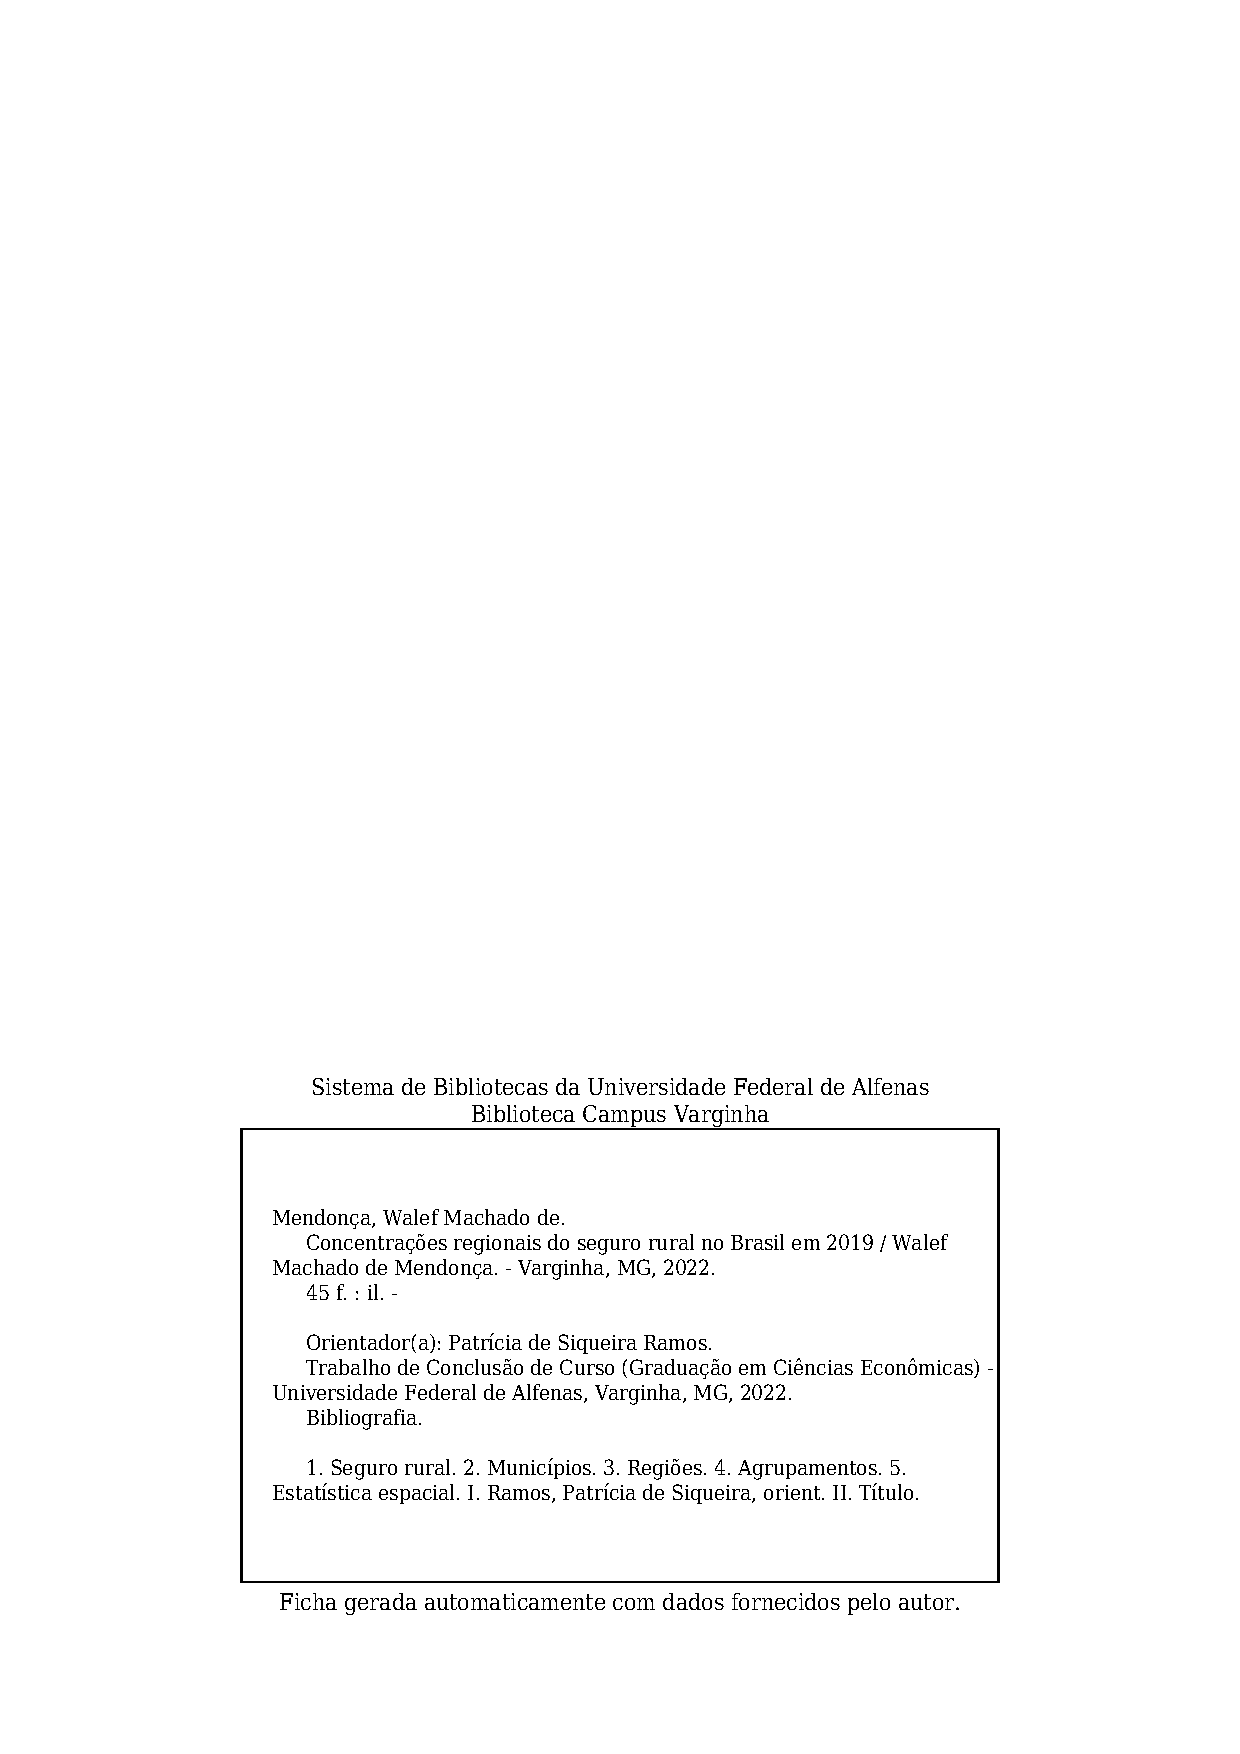
\includepdf{ficha_catalografica.pdf}
\end{fichacatalografica}


%\begin{fichacatalografica}
%	\sffamily
%	\vspace*{\fill}					% Posição vertical
%	\begin{center}					% Minipage Centralizado
%	\fbox{\begin{minipage}[c][8cm]{13.5cm}		% Largura
%	\small
%	\imprimirautor
%	%Sobrenome, Nome do autor
%	
%	\hspace{0.5cm} \imprimirtitulo  / \imprimirautor. --
%	\imprimirlocal, \imprimirdata-
%	
%	\hspace{0.5cm} \thelastpage p. : il. (algumas color.) ; 30 %cm.\\
%	
%	\hspace{0.5cm} %\imprimirorientadorRotulo~\imprimirorientador\\
%	
%	\hspace{0.5cm}
%	\parbox[t]{\textwidth}{\imprimirtipotrabalho~--~\imprimirinstituicao,
%	\imprimirdata.}\\
%	
%	\hspace{0.5cm}
%		1. análise exploratória de dados espaciais.
%		2. $I$ de Moran.
%		2. zoneamento agrícola.
%		I. Patrícia de Siqueira Ramos.
%		II. Universidade Federal de Alfenas.
%		III. Programa de Pós Graduação em Estatística Aplicada e Biometria.
%		IV. A dinâmica espacial da agricultura no Brasil em 2008 e 2018.
%	\end{minipage}}
%	\end{center}
%\end{fichacatalografica}
% ---

% ---
% Inserir errata
% ---
%\begin{errata}
%Elemento opcional da \citeonline[4.2.1.2]{NBR14724:2011}. Exemplo:

%\vspace{\onelineskip}

%FERRIGNO, C. R. A. \textbf{Tratamento de neoplasias ósseas apendiculares com
%reimplantação de enxerto ósseo autólogo autoclavado associado ao plasma
%rico em plaquetas}: estudo crítico na cirurgia de preservação de membro em
%cães. 2011. 128 f. Tese (Livre-Docência) - Faculdade de Medicina Veterinária e
%Zootecnia, Universidade de São Paulo, São Paulo, 2011.

%\begin{table}[htb]
%\center
%\footnotesize
%\begin{tabular}{|p{1.4cm}|p{1cm}|p{3cm}|p{3cm}|}
%  \hline
%   \textbf{Folha} & \textbf{Linha}  & \textbf{Onde se lê}  & \textbf{Leia-se}  \\
%    \hline
%    1 & 10 & auto-conclavo & autoconclavo\\
%   \hline
%\end{tabular}
%\end{table}
%
%\end{errata}
% ---
%%%%%%%%%%%%%%%%%%%%%%%%%%%%%%%%


% ---
% Inserir folha de aprovação
% ---

% Isto é um exemplo de Folha de aprovação, elemento obrigatório da NBR
% 14724/2011 (seção 4.2.1.3). Você pode utilizar este modelo até a aprovação
% do trabalho. Após isso, substitua todo o conteúdo deste arquivo por uma
% imagem da página assinada pela banca com o comando abaixo:
%
% \begin{folhadeaprovacao}
% \includepdf{folhadeaprovacao_final.pdf}
% \end{folhadeaprovacao}
%
%\begin{folhadeaprovacao}
%
% \begin{center}
%    {\ABNTEXchapterfont\bfseries\imprimirautor}
%
%    \vspace*{\fill}\vspace*{\fill}
%    \begin{center}
%      \ABNTEXchapterfont\bfseries\imprimirtitulo
%    \end{center}
%    \vspace*{\fill}
%    
%    \hspace{.45\textwidth}
%    \begin{minipage}{.5\textwidth}
%        A Banca examinadora abaixo-assinada, aprova a Dissertação apresentada como parte dos requisitos para obtenção do título de Mestre em Estatística Aplicada e Biometria pela Universidade Federal de Alfenas. Área de concentração: Ciências Agrárias I.
%    \end{minipage}%
%    \vspace*{\fill}
%   \end{center}
%        
%   Trabalho aprovado. \imprimirlocal, 28 de abril de 2021:
%
%   \assinatura{\textbf{\imprimirorientador} \\ Orientador} 
%   \assinatura{\textbf{Prof. Dr. Lincoln Frias} \\ Coorientador}
%   \assinatura{\textbf{Profª. Drª Adriana Dias} \\ Convidado 1}
%   \assinatura{\textbf{Prof. Dr. Denismar Alves Nogueira} \\ Convidado 2}
   %\assinatura{\textbf{Professor} \\ Convidado 4}
      
%   \begin{center}
%    \vspace*{0.5cm}
%    {\large\imprimirlocal}
%    \par
%    {\large\imprimirdata}
%    \vspace*{1cm}
%  \end{center}
%  
%\end{folhadeaprovacao}
% ---

%\begin{folhadeaprovacao}
%     \includepdf{folha_aprovacao.pdf}
% \end{folhadeaprovacao}




%%%%%%%%%%%%%%%%%%%%
% ---
% Dedicatória
% ---
%\begin{dedicatoria}
%   \vspace*{\fill}
%   \centering
%   \noindent
%    \begin{flushright}
%    \textit{
%    \hspace{8cm} Aos meus pais, Adelvando e Dionísia, e a
%    \hspace{7cm} minha tia Cleonice, por todo amor e cuidado.}
%    \hspace{15cm}\textbf{Dedico este trabalho a vocês.}
%    \end{flushright} 
%\end{dedicatoria}
% ---

% ---
% Agradecimentos
% ---
%\begin{agradecimentos}[\textbf{Agradecimentos}]

%\end{agradecimentos}
% ---

% ---
% Epígrafe
% ---
%\begin{epigrafe}
%    \vspace*{\fill}
%	\begin{flushright}
%		\textit{``Happiness only real \\
%		when shared.'' \\
%		(Christopher McCandless)}
%	\end{flushright}
%\end{epigrafe}
% ---

% ---
% RESUMOS
% ---

% resumo em português
\setlength{\absparsep}{18pt} % ajusta o espaçamento dos parágrafos do resumo
\begin{resumo}[\textbf{Resumo}]
\noindent O ambiente no qual se desenvolvem as atividades agropecuárias apresenta elevado risco e grande incerteza. Variáveis relacionadas aos mercados agropecuários podem gerar oscilações na renda do setor que devem ser enfrentadas por meio de políticas de apoio à gestão de riscos. Uma das formas mais usuais de gerenciamento de risco é a contratação de seguro rural, o qual possibilita a recuperação da capacidade financeira do produtor na ocorrência de sinistros. Destaca-se, no entanto, que o mercado de seguro rural não se consolida sem a participação do Estado devido a problemas como os elevados investimentos e custos administrativos, a possibilidade de riscos catastróficos, e a forte influência do risco moral e da seleção adversa na formação das carteiras. Como mecanismo de estímulo para o desenvolvimento do seguro rural, o governo brasileiro criou o Programa de Subvenção ao Prêmio do Seguro Rural, que divide os custos de aquisição da apólice entre o governo e os produtores. Nesse sentido, o objetivo deste trabalho é agrupar espacialmente os municípios do Brasil segundo variáveis relativas ao seguro rural com o intuito de subsidiar a tomada de decisões em políticas públicas de estímulo à demanda por produtos de seguro específicos para cada grupo de municípios. Para tanto, é apresentado um procedimento para descobrir e explorar padrões de agrupamento espacial com base na distribuição espacial de dados multivariados. Esse procedimento faz uso do algoritmo de agrupamento não hierárquico das k-médias e incorpora a estrutura espacial dos dados através do uso de medidas locais de autocorrelação espacial. A aplicação do procedimento aponta para a existência de maiores concentrações de apólices de seguro rural nas regiões Sul, Centro-Oeste e Sudeste, no sul do Estado de São Paulo. 
   
    \vspace{\onelineskip}
 
   \noindent 
   \textbf{Palavras-chave}: Política agrícola. Zoneamento agrícola. Riscos agropecuários. Autocorrelação espacial.
 
\end{resumo}

% resumo em inglês
\begin{resumo}[\textbf{Abstract}]
 \begin{otherlanguage*}{english}
\noindent  The environment in which agricultural activities are carried out presents high risk and great uncertainty. Variables related to agricultural markets can generate fluctuations in the sector's income that must be addressed through policies to support risk management. One of the most common forms of risk management is the contracting of rural insurance, which makes it possible to recover the producer's financial capacity in the event of accidents. It is noteworthy, however, that the rural insurance market is not consolidated without the participation of the State due to problems such as high investments and administrative costs, the possibility of catastrophic risks, and the strong influence of moral hazard and adverse selection on formation of portfolios. As a mechanism to encourage the development of rural insurance, the Brazilian government created the Subsidy Program for the Rural Insurance Premium, which divides the costs of purchasing the policy between the government and the producers. In this sense, the objective of this work is to spatially group Brazilian municipalities according to variables related to rural insurance in order to support decision-making in public policies to stimulate demand for specific insurance products for each group of municipalities. Therefore, a procedure to discover and explore patterns of spatial clustering based on the spatial distribution of multivariate data is presented. This procedure uses the non-hierarchical k-means clustering algorithm and incorporates the spatial structure of the data through the use of local measures of spatial autocorrelation. The application of the procedure points to the existence of greater concentrations of rural insurance policies in the South, Midwest and Southeast regions, in the south of the State of São Paulo. 


   \vspace{\onelineskip}
 
   \noindent 
   \textbf{Keywords}: Agricultural Policy. Agricultural Zoning. Agricultural risks. Spatial autocorrelation.

 \end{otherlanguage*}
\end{resumo}


% ---
% inserir lista de ilustrações
% ---
\renewcommand{\listfigurename}{\textbf{Lista de Figuras}}
\pdfbookmark[0]{\listfigurename}{lof}
\listoffigures*
\cleardoublepage
% ---

% ---
% inserir lista de quadros
% ---
%\pdfbookmark[0]{\listofquadrosname}{loq}
%\listofquadros*
%\cleardoublepage
% ---

% ---
% inserir lista de tabelas
% ---
\renewcommand{\listtablename}{\textbf{Lista de Tabelas}}
\pdfbookmark[0]{\listtablename}{lot}
\listoftables*
\cleardoublepage
% ---

% ---
% inserir lista de abreviaturas e siglas
% ---
%\begin{siglas}
%  \item[ABNT] Associação Brasileira de Normas Técnicas
%  \item[abnTeX] ABsurdas Normas para TeX
%\end{siglas}
% ---

% ---
% inserir lista de símbolos
% ---
%\begin{simbolos}
%  \item[$ \Gamma $] Letra grega Gama
%  \item[$ \Lambda $] Lambda
%  \item[$ \zeta $] Letra grega minúscula zeta
%  \item[$ \in $] Pertence
%\end{simbolos}
% ---


% ---
% inserir o sumario
% ---
\renewcommand\contentsname{\textbf{Sumário}}
\pdfbookmark[0]{\contentsname}{toc}
\tableofcontents*
\cleardoublepage
% ---



% ---
% Ajustar nomes em negrito
% ---
\renewcommand{\resumoname}{\textbf{RESUMO}}
%\renewcommand{\tableofcontentsname}{\textbf{SUMÁRIO}}




% ----------------------------------------------------------
% ELEMENTOS TEXTUAIS
% ----------------------------------------------------------
\textual
\pagestyle{simple}     %Remover o cabeçalho

\setcounter{page}{6}   %Ajustar a númeração da página (Capa e Ficha Catalográfica não são contadas)


%Introdução ====================================================================
\newpage
\section{\textbf{INTRODUÇÃO}}

A contratação de seguro rural é uma das formas mais frequentes de gerenciamento de riscos agropecuários. Essa forma de seguro opera com o objetivo de atenuar as perdas e viabilizar a recuperação da capacidade financeira do produtor na ocorrência de sinistros. O seguro rural também promove um ambiente mais propício ao desenvolvimento das atividades agropecuárias, pois proporciona a garantia do fluxo de renda, contribui para um aumento da área plantada e facilita a obtenção de financiamento. Além disso, ele se apresenta como um instrumento que promove o compartilhamento do risco da agropecuária com outros agentes e setores econômicos da sociedade \cite{brasil19}.

É importante destacar que o mercado de seguro rural não se consolida sem a participação do Estado. O ambiente de elevado risco e considerável incerteza no qual se desenvolvem as atividades agropecuárias impõe a existência de fatores que limitam a eficiência da iniciativa privada na oferta de produtos de seguro rural. Destacam-se problemas como os elevados investimentos e custos administrativos, a possibilidade de riscos catastróficos, a forte influência do risco moral e da seleção adversa na formação das carteiras, como fatores que limitam a eficiência da iniciativa privada na oferta do seguro rural. 

Os principais riscos agropecuários se devem, principalmente, às instabilidades climáticas e ameaças sanitárias, que podem afetar a produção, ou a razões de mercado, como variações das taxas de câmbio e juros, ou a condições ligadas ao ambiente de negócios, tais como alterações em marcos regulatórios e em políticas públicas. Todas essas variáveis, relacionadas aos mercados agropecuários, geram variações na renda do setor, que devem ser enfrentadas através de políticas de gerenciamento de gestão de riscos (BRASIL, 2018). Nesse sentido, o poder público é demandado a interferir no mercado, seja atuando diretamente como seguradora, seja criando programas que estimulem a oferta e a demanda por produtos de seguro.

Uma das formas utilizadas como mecanismo de estímulo ao desenvolvimento do seguro rural no Brasil, é o Programa de Subvenção ao Prêmio do Seguro Rural (PSR), instituído pela Lei 10.823/2003 e decreto nº 5.121/2004 (BRASIL, 2018). Esta política do governo brasileiro tem como objetivo tornar o seguro rural mais barato para os produtores rurais, dividindo os custos de aquisição da apólice entre o governo e os produtores. 

Neste contexto, este trabalho busca identificar grupos de municípios com características semelhantes em relação à adesão ao seguro rural através do agrupamento de dados multivariados com base em medidas locais de autocorrelação espacial. Isso faz com  que os agrupamentos obtidos levem em consideração não apenas o valor das variáveis de seguro rural, mas também seu posicionamento geográfico. Dessa forma, busca-se auxiliar na tomada de decisões sobre políticas públicas de estímulo à demanda por produtos de seguro específicas para cada grupo de municípios. 

Para tanto, é apresentado um procedimento para descobrir e explorar padrões de agrupamento espacial com base na distribuição espacial de dados multivariados. Esse procedimento faz uso do algoritmo de agrupamento não hierárquico das k-médias e incorpora a estrutura espacial dos dados através do uso de medidas locais de autocorrelação espacial como o \textit{I} de Moran local e \textit{G} de Getis e Ord local. 


%Referencial teórico ====================================================================
%\newpage
\section{\textbf{REFERENCIAL TEÓRICO}}\label{referencial}

\subsection{SEGURO RURAL}

De acordo com o Guia de Seguros Rurais\footnote{Elaborado pela Comissão Nacional de Política Agrícola da Confederação da Agricultura e Pecuária do Brasil (CNA) e pelo Ministério da Agricultura, Pecuária e Abastecimento (MAPA).}, a ocorrência de sinistros devido a eventos climáticos adversos tem provocado prejuízos consideráveis para agricultores, mesmo tendo em conta o elevado nível tecnológico empregado nas atividades agropecuárias (GUIA DE SEGUROS RURAIS, 2020). 

A ocorrência desses sinistros se deve ao fato de que as atividades do setor agropecuário são dotadas de especificidades em relação à dimensão dos riscos aos quais estão expostas. Os principais riscos estão associados aos aspectos biológicos da produção e sua interdependência com os fatores climáticos \cite{burgo05}. Também se destacam os riscos associados à volatilidade dos preços, assim como variações das taxas de juros e de câmbio. Dessa forma, os riscos e incertezas inerentes à produção agropecuária podem causar perdas econômicas que têm potencial de afetar não apenas os produtores rurais como toda a sociedade \cite{brasil19b}. 

% DEFINIÇÃO DE SEGURO RURAL...
Este contexto torna evidente a necessidade de medidas de gestão de risco como a contratação do seguro rural. De um modo geral, o seguro caracteriza-se pela transferência das consequências econômicas, da realização de um determinado risco, do segurado para a seguradora. O mesmo ocorre com o seguro rural, cujo papel é reduzir riscos e proteger a renda dos produtores rurais \cite{guia20, brasil21}.

Um sistema de seguridade rural eficiente tem como principal vantagem garantir ao produtor a segurança necessária para continuar a investir na produção e se manter competitivo no setor agropecuário mesmo em situações de ocorrência de adversidades climáticas, que ocasionam perda patrimonial ou da safra. Dessa forma, o seguro rural se apresenta como um importante recurso para estabelecer uma proteção à renda dos produtores \cite{guia20}. 

Além do mais, do ponto de vista dos efeitos agregados, o seguro rural desempenha um papel importante, pois proporciona um bom ambiente de desenvolvimento para a agricultura. O seguro rural auxilia na oferta de financiamento, promove o crescimento da área plantada e é uma ferramenta que pode compartilhar os riscos agrícolas com os demais agentes e setores da economia \cite{brasil21}.

% DESAFIO DO SEGURO RURAL
Contudo, é importante destacar que o desenvolvimento de um sistema de seguro rural é em si um desafio devido à natureza dos riscos da atividade agropecuária. Por exemplo, há uma dependência espacial na ocorrência de eventos climáticos adversos, o que faz com que o seguro rural contrarie a suposição de que, em um seguro, o risco agregado deve ser menor que o risco individual. Fatores como este fazem com que as seguradoras tenham dificuldade em constituir carteiras que viabilizem a diversificação dos riscos \cite{barros12, fornazier12}

Associados aos altos custos operacionais e a dificuldades em uma precificação que leve em conta a dependência e heterogeneidade dos sinistros, é importante destacar que elementos como a assimetria de informação e o risco moral, devido à ausência de dados históricos dos produtores, prejudicam a atividade das empresas de seguro rural. Isso acontece porque, diante deste cenário, as seguradoras que atuam no seguro rural acabam cobrando valores altos para os prêmios, o que causa um desincentivo à aderência ao seguro. Dessa forma, ressalta-se que as subvenções concedidas pelo governo desempenham um atribuição essencial, pois, ao tornar viável a cobertura para o produtor rural, buscam corrigir as falhas de mercado e proporcionar a expansão da área segurada \cite{guimaraes09, barros12}.

% Reescrever a partir aqui
\subsubsection{O Seguro Rural no Brasil}

As primeiras tentativas de implantar o seguro rural no Brasil se passaram na década de $1930$ no estado de São Paulo. A criação, em $1939$, de um seguro obrigatório que oferecia proteção contra o granizo na produção de algodão foi uma das iniciativas pioneiras no estado de São Paulo \cite{maia11}. A partir de então, os resultados positivos alcançados pelo seguro para a proteção da lavoura do algodão inspiraram a criação de novos programas como a Carteira de Seguro Agrícola contra Granizo para a Viticultura, instituída em $1948$, e a Carteira de Seguro Agrícola contra Geada para Horticultura criada em $1964$ \cite{silva14}.

No final da década de $1940$, foi criado no Instituto Rio-Grandense do Arroz (Irga) o seguro para granizo e o seguro para indenizar os produtores de fumo nos estados de Santa Catarina e Rio Grande do Sul, criado pela Associação dos Fumicultores do Brasil (Afubra) e mantido com recursos próprios \cite{silva14}. 

Além disso, em $1948$, foi criado, no âmbito federal, o Instituto de  Resseguros do Brasil (IRB), que tinha como objetivo reduzir os prejuízos causados por eventos adversos e assegurar maior estabilidade aos produtores rurais \cite{silva14}. Também foi fundada em $1954$, pelo Governo Federal, a Companhia Nacional de Seguro Agrícola (CNSA) e o Fundo de Estabilidade do Seguro Agrário. Segundo, Maia,  Roitman e de Conti (2011), a estruturação e gestão dos seguros da CNSA ficaram sob responsabilidade do IRB. Contudo, as atividades da CNSA foram finalizadas em $1996$, em decorrência, segundo Gemignani (2000), da incapacidade em difundir o seguro rural de forma a tornar possível sua viabilização econômica \cite{maia11, silva14}.

Segundo Silva, Teixeira e Santos (2014), o Decreto-Lei nº $73$ de $1966$ e o Decreto nº $60.459$ de $1967$ estabelecem as bases legais para as atividades de seguro e a criação do Sistema Nacional de Seguros Privados (SNSP). Com o decreto de $1967$ também foi instituído o Fundo de Estabilidade do Seguro Rural (FESR), cujos recursos eram geridos pelo IRB e a principal função era garantir a estabilidade das operações de seguro e proporcionar uma proteção complementar para os riscos de sinistro \cite{silva14}

Com um papel importante na definição das modalidades de seguros agrários, a Resolução nº $5$ do Conselho Nacional de Seguros Privados foi instituída em $1970$. Essa resolução define que o seguro agrícola deve fornecer cobertura contra perdas decorrentes de fenômenos meteorológicos, doenças e pragas. Além disso, no setor pecuário, o seguro deve fornecer cobertura para mortes de animais causadas por doenças ou acidentes, assim como o seguro de benfeitorias e produtos agropecuários. Por fim, a Resolução nº $5$ também estabelece o seguro de crédito, que cobre incapacidade de pagamento de compradores dos produtos agropecuários \cite{silva14}.

Apesar das várias ações implementadas pelo Governo Federal, o seguro rural evoluiu de forma lenta e limitada a uma reduzida parcela da produção. Os problemas do desenvolvimento do seguro rural  motivaram a criação do Programa de Garantia da Atividade Agropecuária (Proagro), através da Lei nº $5.969$, de $11$ de dezembro de $1973$ \cite{silva14}. Inicialmente, o programa ficou sob a responsabilidade do Banco Central, que passou a vincular o seguro rural às operações de crédito agropecuário e utilizou emissões monetárias para pagamentos de sinistros. Segundo Maia, Roitman e De Conti (2011), o sistema de financiamento do Proagro gerou déficits que motivaram diversas modificações no Programa, que ainda continua sendo um dos mais importantes instrumentos para a gestão de riscos na agricultura no Brasil \cite{maia11}.

% reescrever a partir daqui 
A partir de $2003$, o Governo Federal começou a adotar uma política de subvenção através do Programa de Subvenção ao Prêmio do Seguro Rural (PSR), instituído por meio da Lei nº 10.823 de $19$ de dezembro de $2003$. Este programa objetiva, assim como ocorre com seguros rurais em países europeus e nos Estados Unidos, conceder subvenção econômica ao valor do prêmio do seguro rural contratado com seguradoras autorizadas \cite{maia11, silva14}.

\subsubsection{Programas de Subvenção ao Prêmio do Seguro Rural}

O PSR foi instituído pelo Decreto nº 5.121 de 2004 e tem a finalidade de subsidiar parte do prêmio do seguro rural, de forma a garantir o papel do seguro rural como mecanismo de estabilidade da renda do produtor, além de propor a aplicação das tecnologias adequadas para os empreendimentos agropecuários \cite{guia20}

A operacionalização do PSR é feita pelo Ministério da Agricultura, Pecuária e Abastecimento (MAPA). Nesse programa, os produtores rurais que devem fazer a contratação do seguro rural diretamente com as seguradoras habilitadas pela Superintendência de Seguros Privados (Susep) e cadastradas no MAPA. Assim, para obter os recursos do programa, os produtores devem contratar a apólice e requerer a subvenção do governo federal. Por sua vez, o governo federal repassa para as seguradoras habilitadas um percentual do prêmio do seguro contratado, resultando na redução do valor a ser pago pelo produtor rural \cite{silva14}.

As técnicas de execução e prioridades da política do PSR são estabelecidas pelo Comitê Gestor Interministerial do Seguro Rural (CGSR). Com o objetivo de fiscalizar a gestão do programa, o CGSR é formado pelo MAPA, que é responsável pela coordenação, e por representantes do Ministério da Economia (ME) e da Superintendência de Seguros Privados (Susep). Dessa forma, o valor de subvenção ao prêmio do seguro rural leva em conta algumas características como a modalidade do seguro, o tipo de cultura e o tipo de cobertura \cite{brasil21}.

É necessário destacar que, conforme apresentado no Guia de Seguros Rurais (2020), o PSR tem como condição o cumprimento dos indicadores do Zoneamento Agrícola de Risco Climático (ZARC) para o recebimento da subvenção. O ZARC  é um levantamento do período de plantio das culturas por município e considera características como o tipo de solo e o clima da região. Dessa forma, o ZARC busca evitar que eventos climáticos adversos ocorram durante as fases em que as culturas se encontram mais expostas e, com isso, reduzir as perdas \cite{guia20}.

Diante da relevância do setor agrícola para a economia brasileira, é possível entender que o seguro rural e o PSR são importantes formas de gestão de risco e que colaboram para uma agricultura mais eficiente e com riscos reduzidos para o produtor rural. Isso vale especialmente para o PSR, que opera como uma forma de fomentar a aquisição das apólices de seguro rural, objetivando induzir o uso de tecnologias adequadas e modernizando a gestão do empreendimento agropecuário. 

% Dessa forma, como este estudo propõe-se a analisar a distribuição e a presença de dependência ou heterogeneidade espacial de dados multivariados do seguro rural nos municípios brasileiros entre os anos de $2006$ e $2019$, a próxima seção apresenta a metodologia da Análise de Componentes Principais (ACP) e da Análise Exploratória de Dados Espaciais (AEDE).


% Reescrever daqui...

\subsection{ANÁLISE ESPACIAL}

A análise espacial consiste em um conjunto de técnicas destinadas a incorporar o espaço à análise. Ou seja, a análise espacial, constitui-se de métodos capazes de mensurar propriedades e relações baseados na localização espacial de um determinado fenômeno. Portanto, antes de iniciar a modelagem, muitas vezes é efetuada uma análise exploratória de dados para localizar padrões de dependência espacial no fenômeno em estudo \cite{camara04}.

Os principais fenômenos abordados na análise espacial incluem a dependência espacial e a heterogeneidade espacial. O fenômeno da dependência espacial pode ser representado pela primeira lei da geografia ou pela lei de Tobler. O geógrafo suíço Waldo Tobler apresentou a lei no ano de 1970, afirmando que tudo depende de tudo, mas as coisas que estão mais próximas estão mais relacionadas entre si do que coisas mais distantes. Portanto, a dependência espacial estabelece que o valor de uma variável em uma determinada região depende do valor da mesma variável em uma região próxima \cite{almeida12}.

Dessa forma, segundo Almeida (2012), processos temporais apresentam relações diferentes dos processos espaciais. O que quer dizer que, nos processos temporais, o valor de uma variável qualquer no tempo $t$ é influenciado pelo valor da variável no tempo $t-1$, mas o inverso não ocorre. Em contraste a esse tipo de processo, nos  processos espaciais têm-se a multidirecionalidade nas relações entre as regiões, ou seja, o valor da variável na região $i$ depende do valor na região $j$, e a região $j$ depende da região $i$ em relação ao valor da mesma variável.

%Heterogeneidade Espacial

%O relacionamentos espaciais incorporados à análise, a heterogenidade espacial, refere-se à variação nos relacionamentos entre as variáveis ao longo do espaço. Em geral, podem-se esperar diferentes relacionamentos em cada uma das unidades espaciais, podendo a relação linear entre tais unidades ser escrita como:

%\begin{align*}
%y_i = X_i \beta_ i + \epsilon_i,
%\end{align*}

%$\noindent em que $i$ é o índice da observação no espaço, assumindo valores de 1 a \textit{n}, $X_i$ representa o vetor contendo os \textit{k} valores da variável explicativa, tendo um conjunto de parâmetros associados $\beta_i$.

%É importante ressaltar que os dados espaciais possuem alguns problemas que podem ser danosos à análise. Além da heterogeneidade espacial e da dependência espacial, é possível citar problemas como a falácia ecológica, o problema da unidade de área modificável, o efeito de beirada e a influência de \textit{outliers} espaciais. 

%De acordo com Almeida (2012), a falácia ecológica está relacionada com erros que se originam ao deduzir o comportamento do indivíduo através análise de dados agregados. Almeida (2012) argumenta que há razões para inferir, ainda que parcialmente, comportamentos individuais por meio de dados agregados. Uma situação possível é quando alguns comportamentos individuais são influenciados pelo comportamento do grupo. No entanto, via de regra, as concluões a respeito de comportamento individual devem se basear primordialmente em dados individuais. 
 
%Outro problema que surge no contexto da análise espacial é o  problema de unidade de área modificável, usualmente denotado pela sigla MAUP, do inglês \textit{modifiable areal unit problem}. Esse problema se refere, basicamente as consequencias causadas pelas diferentes formas de se delimitar as unidades espaciais. A necessidade de agregação de informações espaciais se dá pela ausência de dados individuais, ou então quando as unidades agregadas são o objeto da análise.

%Segundo Haining (2003), o MAUP apresenta dois efeitos distintos, o problema de escala e o de partição. O primeiro deles se relaciona à escala da análise, ou seja, ao número de subáreas em que a região de estudo foi particionada. O número de partições determina também o tamanho de cada unidade espacial nas quais os eventos são observados, portanto é capaz de influênciar o resultado de estatísticas. O segundo efeito diz respeito a forma das partição das unidades, ou seja, como as  áreas estão divididas mantendo-se constante o  o número de áreas.

%O efeito de beirada se deve a possibilidade da dependência espacial ir além das fronteiras da região de estudo, podendo o valor da variável mensurada depender de outras unidades espaciais que não fazem parte da mesma (ANSELIN, 1988). Tal efeito interfere na  inferência estatística de modelos de processos espaciais. Aĺém disso, Almeida (2012) aponta que, por terem um menor número de regiões vizinhas, as regiões da fronteira também fornecem menos informação para a construção de valores médios, como por exemplo as defasagens espaciais.

%Para lidar com o efeito beirada, Griffith (1983) propôs a criação de vizinhos artificiais para as regiões de fronteira por meio da replicação do mapa. Desta forma, as regiões da beirada oposta da área de estudo seriam também vizinhas da outra beirada. Porém, como destacado por Darmofal (2006) a dúvida seria saber se tais vizinhos artificiais realmente apresentam interação espacial com a região. Outra solução apontada por Almeida (2012) seria estender a área de estudos, considerando adicionalmente uma zona ao longo de toda a fronteira.

%Outliers e pontos de alavancagem
Além disso, é necessário destacar, entre os objetivos da análise espacial, a investigação da presença dos \textit{outliers} espaciais. Os \textit{outliers} são definidos como valores extremos com relação a suas posições no espaço geográfico. A presença de \textit{outliers} espaciais ocorre levando-se em consideração a diferença entre os valores em relação ao conjunto de valores das regiões vizinhas \cite{haining03}. Os \textit{outliers} espaciais podem surgir do processo de obtenção e armazenamento dos dados, no entanto, tais valores podem apontar para a existência de valores extremos e representar atributos do fenômeno analisado. Portanto, a presença de \textit{outliers} espaciais impõe a necessidade de uma investigação mais cuidadosa \cite{almeida12}.

\subsubsection{Matriz de ponderação espacial}

Em uma matriz de ponderação espacial, ou matriz de pesos espaciais, cada conexão entre duas regiões é representada por uma entrada na matriz que é denominada peso espacial. Essa matriz tem como objetivo representar um determinado arranjo espacial das interações resultantes de um fenômeno em estudo \cite{almeida12}. A matriz de ponderação espacial tem dimensão $n \times n$ e é, usualmente, denotada por $\boldsymbol{W}$: 

\begin{align*}
	\boldsymbol{W} =
	\left[
	\begin{array}{cccc}
		w_{11} & w_{12} & \dots & w_{1n} \\
		w_{21} & w_{22} & \dots &w_{2n} \\
		\vdots & \vdots & \ddots & \vdots \\
		w_{n1} & w_{n2} & \dots & w_{nn}\\
	\end{array}
	\right],
\end{align*}

\noindent em que $n$ é o número de regiões em análise. Cada elemento $w_{ij}$ retrata uma medida de proximidade entre as áreas $i$ e $j$ \cite{camara04}. 

É possível enumerar dois problemas com a atribuição da matriz de ponderação espacial a ser utilizada. Primeiramente, é possível que a escolha da matriz $\boldsymbol{W}$ seja arbitrária, uma vez que não existe teste formal para sua escolha. Além disso, há o problema que se relaciona à sensibilidade dos resultados à escolha da matriz. Dessa forma, a escolha da matriz de ponderação espacial possuí fundamental relevância e, portanto, deve ser feita com uma fundamentação teórica \cite{almeida12}. 

Os modelos tradicionais comumente utilizam, em sua maioria, características físicas e geográficos para determinar um critério de distâncias entre as regiões. Os critérios de vizinhança, distância geográfica ou de tempo de deslocamento são os mais utilizados. No entanto, é possível que a matriz de pesos espaciais utilize como critério de distâncias entre as regiões os aspectos socioeconômicos \cite{tyszler06}. 

Uma matriz comumente utilizada é a matriz de ponderação espacial por contiguidade. Nessa matriz, são levadas em consideração as fronteiras físicas em comum entre duas regiões. Se duas regiões apresentam relação de vizinhança, é atribuído ao elemento correspondente na matriz o valor $1$, caso contrário é atribuído o valor $0$. Formalmente, tem-se:

\[
w_{ij} = 
\begin{cases}
\text{1,} & \quad\text{se $i$ e $j$ são contíguos} \\
\text{0,} & \quad\text{se $i$ e $j$ não são contíguos.}\\
\end{cases}
\]
\\

Destaca-se que convencionou-se assumir que $w_{ij} =  0$, para todo $i = j$, ou seja, uma determinada região não é considerada vizinha de si própria. Porém, embora com menor frequência, é possível encontrar na literatura regiões sendo vizinhas de si mesmas. %Além disso, o conceito de fronteira geográfica pode apresentar diferentes definições na observação de um mapa, para isso, o movimento de peças em um tabuleiro de xadrez é utilizado para denominar algumas das diferentes convenções de contiguidade \cite{almeida12}

%Na Figura \ref{contiguidade} são representadas três diferentes convenções de continguidade: rainha (\textit{queen}), torre (\textit{rook}) e bispo (\textit{bishop}), respectivamente. Na primeira delas, além das regiões que fazem fronteira com a região $A$, os vértices são considerados vizinhos. Na convenção torre, apenas as regiões que fazem fronteira com a região são consideradas vizinhas de $B$. No último caso, apenas os vértices são considerados vizinhos da região $C$.

%\begin{figure}[h!]
%	\centering
%	\small
%	\subfloat[Rainha\label{fig:a}]{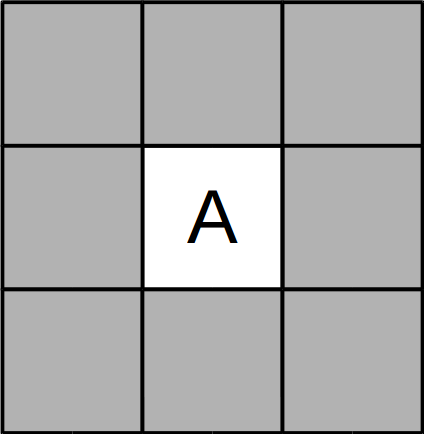
\includegraphics[width=0.15\textwidth]{img/cont_queen.png}}\hspace{0.2cm}
%	\subfloat[Torre\label{fig:b}]{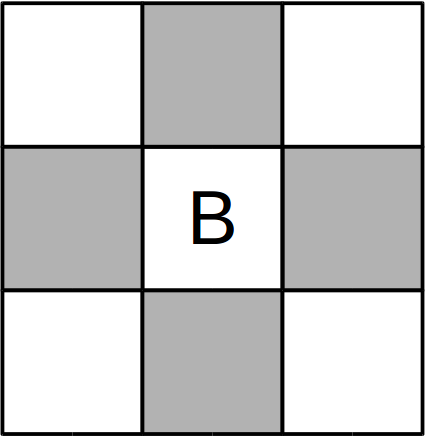
\includegraphics[width=0.15\textwidth]{img/cont_rook.png}}\hspace{0.2cm}
%	\subfloat[Bispo\label{fig:c}]{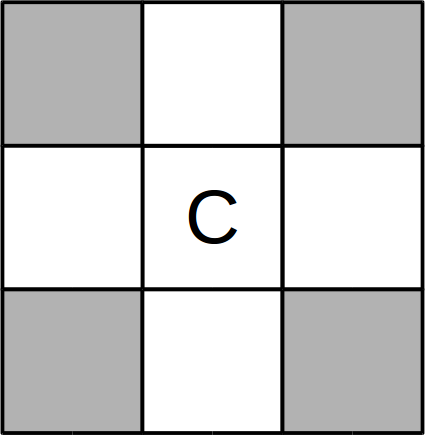
\includegraphics[width=0.15\textwidth]{img/cont_bishop.png}}
%	\caption{Convenções de contiguidade}
%	\small \textsuperscript {Fonte: Elaboração própria}
%	\label{contiguidade}
%\end{figure}


É necessário ressaltar que a matriz de contiguidade binária é simétrica, de forma que se duas regiões $i$ e $j$ possuem fronteiras físicas em comum, tanto $w_{ij}$ quanto $w_{ji}$ serão iguais a 1. Assim, a influência exercida pela região $i$ em $j$ será observada na relação entre $j$ e $i$, o que representa formalmente o conceito de multidirecionalidade da influência espacial. Um fato a se destacar é que, normalmente é realizada a normalização da matriz de ponderação espacial, ou seja, divide-se o valor de cada elemento da matriz $\boldsymbol{W}$ pelo valor da soma dos valores da linha em que ele se encontra. Uma vez realizada a normalização, a matriz resultante não será  necessariamente simétrica. 

%As matrizes que utilizam as distâncias geográficas como critério para a definição dos pesos consideram que duas regiões próximas geograficamente apresentam maior interação espacial. Dentre as matrizes com essa definição, a matriz dos $k$ vizinhos mais próximos é uma das mais utilizadas. Na Equação \ref{W_prox}, $d_i(k)$ representa a menor distância em relação a região $i$ para que $i$ tenha exatamente $k$ vizinhos \cite{almeida12}.

%\begin{align}
%	w_{ij} = 
%	\begin{cases}
%		\text{$1,$} & \quad\text{se $d_{ij} < d_i(k)$} \\
%		\text{$0,$} & \quad\text{se $d_{ij} > d_i(k)$}\\
%	\end{cases}
%	\label{W_prox}
%\end{align}

%De acordo com Almeida (2012), a matriz de pesos espaciais gerais de Cliff e Ord  estabelece que, duas regiões que compartilham maior extensão de fronteira apresentam uma maior interação entre si, além de considerar o fator de distância entre as regiões. Ambas as informações são utilizadas no cálculo dos pesos da matriz, sendo esses definidos pelo comprimento relativo da fronteira comum entre as regiões, ajustados pela distância inversa entre elas. Os pesos espaciais da matriz de pesos gerais são expressos da seguinte maneira:
 
%\begin{align*}
%w_{ij} = \frac{f_{ij}^\phi}{d_{ij}^\delta},
%\end{align*}

%\noindent em que $f_{ij}$ é a proporção da fronteira comum entre as observações $i$ e $j$ no perímetro de $i$, e $\phi$ e $\delta$ são parâmetros a serem definidos. Tal matriz de pesos espaciais não necessariamente será simétrica. Ao levar em consideração a proporção do perímetro total da região $i$ que é comum a região $j$ em regiões de diferentes perímetros, tal proporção também seria distinta.

\subsubsection{Análise exploratória de dados espaciais}


Com o objetivo de descrever como estão distribuídas espacialmente as observações, a análise exploratória de dados espaciais (AEDE) busca compreender os padrões de associação espacial e verificar a existência de \textit{clusters} espaciais. Além disso, essa metodologia  objetiva analisar a existência de diferentes regimes espaciais  ou outras formas de instabilidade, identificação de observações atípicas, ou como são também denominados, \textit{outliers} espaciais \cite{almeida12}.

A necessidade de se fazer uso de metodologias que considerem a distribuição espacial se dá pois a identificação de padrões de associação espacial pela percepção humana tende a criar padrões viesados. Ou seja, é possível que em uma análise menos criteriosa encontrem-se padrões até mesmo em dados distribuídos de forma aleatória \cite{messner99}. Através dessas metodologias, podem-se utilizar indicadores de associação espacial globais ou locais com o objetivo de identificar os diferentes regimes espaciais do conjunto de dados.

A Figura \ref{autocorrelacao} apresenta exemplos de padrões de autocorrelação espacial. Pode-se identificar em  \subref{autocorrelacao:a} um padrão de autocorrelação positivo, ou seja, valores semelhantes estão localizados próximos uns dos outros. Em  \subref{autocorrelacao:b} é apresentado um padrão de autocorrelação nula, o que indica que há aleatoriedade na distribuição espacial. Por sua vez, em \subref{autocorrelacao:c}, há um padrão de autocorrelação negativa, assinalando que valores dissimilares localizam-se próximos uns dos outros. 

\begin{figure}[!htb]
	\caption{Padrões de autocorrelação espacial}\label{autocorrelacao}
	\begin{center}
    	\subfigure[Positiva\label{autocorrelacao:a}]{
    	
\includegraphics[width = 0.2\linewidth]{img/autocor_pos.png}}
    	\subfigure[Nula\label{autocorrelacao:b}]{
    	
\includegraphics[width = 0.2\linewidth]{img/autocor_null.png}}
    	\subfigure[Negativa\label{autocorrelacao:c}]{
    	
\includegraphics[width = 0.2\linewidth]{img/autocor_neg.png}}
	\end{center}
	\noindent Fonte: Elaboração própria
\end{figure}

Em contraste à Figura \ref{autocorrelacao}, que apresenta dados no formato de grades regulares, geralmente as regiões em estudo são polígonos irregulares. Esse fato  prejudica a identificação visual dos padrões de autocorrelação espacial (principalmente autocorrelação nula e negativa). Portanto, é necessário lançar mão de testes estatísticos para a identificação dos padrões de autocorrelação espacial.

\subsubsection{Autocorrelação espacial global}

Um dos principais indicadores de autocorrelação espacial global é o coeficiente I de Moran \cite{almeida12}. Este coeficiente é definido através de uma medida de autocovariância na forma de produto cruzado. Algebricamente a estatística é dada por:

\begin{align}
\label{IMoran}
I = \dfrac{n}{S_0} \dfrac{\sum_{i} \sum_{j} w_{ij} z_i z_j}{\sum_{i=1}^{n} z_i^2},
\end{align}

\noindent em que $n$ retrata o número de regiões, $z_i$ indica o valor da variável de interesse padronizada na região $i$ e $S_0$ representa o somatório de todos os pesos espaciais da matriz $\boldsymbol{W}$ \cite{almeida12}:

%O \textit{I} de Moran pode ser calculado matricialmente da seguinte forma:

%\begin{align*}
%I = \dfrac{n}{S_0} \dfrac{z'\boldsymbol{W}z}{z'z},
%\end{align*}

%\noindent em que $\boldsymbol{W}z$ denota os valores médios da variável padronizada nos vizinhos de acordo com a matriz $\boldsymbol{W}$.

De forma geral, o \textit{I} de Moran é utilizado para testar a existência de autocorrelação espacial e, nesse contexto, a aleatoriedade espacial é a hipótese nula. Cliff e Ord \cite{cliff81} demonstraram que o \textit{I} de Moran não é centrado em $0$, mas sim em seu valor esperado $-[1/(n-1)]$, que é o valor que seria obtido em um cenário de distribuição espacial aleatória. Assim, valores do \textit{I} de Moran entre o valor esperado e $1$ indicam a presença de autocorrelação espacial positiva, valores entre $-1$ e o valor esperado apontam para a presença de autocorrelação espacial negativa. 

A autocorrelação espacial positiva revela que as regiões que apresentam valores altos (acima da média) da variável de interesse tendem a ter ao seu redor regiões que também apresentam valores altos (acima da média) desta variável e regiões com baixos valores (abaixo da média) tendem a estar rodeadas por regiões que também apresentam baixos valores (abaixo da média). Em contraste, a autocorrelação espacial negativa aponta a  dissimilaridade entre os valores da variável e a sua localização. Nesse sentido, geralmente regiões com valores altos da variável estão circundadas por regiões com baixos valores e regiões com baixos valores têm em seu entorno regiões com valores altos \cite{almeida12}.

A verificação da significância do valor do índice I de Moran pode ser obtida pela associação do índice a uma distribuição estatística, geralmente a distribuição normal. A forma mais utilizada para tal verificação é o teste de pseudo-significância ou, como também é conhecido, teste de permutação aleatória. Esse teste não possui pressupostos em relação à distribuição e nesta abordagem são geradas diferentes permutações dos valores associados às regiões, produzindo para cada permutação um novo arranjo espacial com os valores redistribuídos entre as áreas. Dado que o cenário real observado corresponde somente a apenas um dos arranjos, tem-se uma distribuição empírica do índice \cite{camara04}. 

Outra forma de visualizar os regimes espaciais é o diagrama de dispersão de Moran, exemplificado na Figura \ref{dispersaomoran}. No eixo horizontal do diagrama de dispersão de Moran, são retratados os valores padronizados da variável de interesse, já o eixo vertical apresenta as médias da variável nos vizinhos das respectivas áreas, também conhecidas como defasagens espaciais. 

\begin{figure}[h!]
	\centering
	\caption{Diagrama de dispersão de Moran}\label{dispersaomoran}
	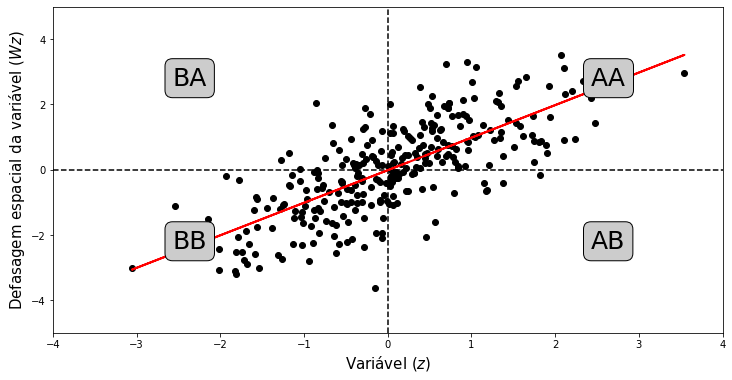
\includegraphics[scale = 0.4]{img/moran_scatter.png}\\
	%\vspace{-0.4cm}
	\small \textsuperscript {Elaboração própria com dados simulados.}
\end{figure}

\subsubsection{Autocorrelação espacial local}

%%%%%%%%%%%%%%% G de Getis & Ord  %%%%%%%%%%%%%%% 

Um indicador de concentração com a capacidade de analisar localmente a associação espacial foi inicialmente apresentado por Getis e Ord em $1992$ \cite{almeida12}. De acordo com Getis e Ord (1992), essa estatística indica a presença de eventuais agrupamentos localizados de concentração espacial, chamados de \textit{hot spots} e \textit{cool spots}. A estatística  denota, para cada observação $i$, em que medida essa observação está rodeada por valores altos (\textit{hot spot}) ou baixos (\textit{cool spot}). Para uma determinada variável $y$, a estatística é calculada da seguinte forma:

\begin{equation}
G_i(d) = \dfrac{\sum_{j} w_{ij}(d) y_j}{\sum_{j}  y_j},\quad \text{para  $j \neq i$}.
\label{g_getis_ord}
\end{equation}

O somatório em $j$ faz com que apenas os valores dos vizinhos próximos da região $i$ sejam utilizados no cálculo da estatística. A matriz de ponderação espacial $\boldsymbol{W}$ pode ou não ser uma matriz de proximidade geográfica, baseada em um raio construído em torno da região $i$.

A estatística $G$ de Getis e Ord possui duas formulações possíveis. Se não incluir a observação sob consideração $i$, tem-se a estatística $G_i$ como apresentada da definição \ref{g_getis_ord}. Se incluir a observação $i$ no somatório, obtém-se $G_i^*$, que é expressa como: 

\begin{equation}
G^*(d) = \dfrac{\sum_{j} w_{ij}(d) y_j}{\sum_{j}  y_j},\quad \text{para qualquer } j.
\label{g_getis_ord_s}
\end{equation}

A média da estatística $G_i$ é dada por 

\begin{equation*}
\mathbb{E}(G) = \dfrac{W_i}{(n-1)}  
\end{equation*}

\noindent em que $W_i = \sum_j x_{ij}(d)$

A variância da estatística $G_i$ é dada por  

\begin{equation}
	Var(G_i)= \dfrac{W_i(n-1-W_i)}{(n-1)^2(n-1)} \bigg[\dfrac{s(i)}{\bar{y}(i)}\bigg]^2
\end{equation}

\noindent em que $\bar{y}(i)= \dfrac{\sum_j y_j}{(n-1)}$ e $s^2(i) = \dfrac{\sum_j y_j^2}{(n-1)} - [\bar{y}(i)]^2$. 

A interpretação da estatística $G$ é feita com base no sinal de $Z(G_i)$, valores positivos e significativos indicam um \textit{cluster} espacial do tipo \textit{hot spot}, ou seja, com valores altos para a variável de interesse. Por outro lado, um valor negativo e significativo de $Z(G_i)$ indica um \textit{cluster} do tipo \textit{cool spot}, ou seja de baixos valores para a variável de interesse. A inferência a respeito da significância da estatística $G_i$ é baseada na normal padrão, ou seja, $Z(G_i)$ \cite{almeida12}. 

Ressalta-se, ainda, que o indicador proposto por Getis e Ord não é capaz de revelar uma situação de correlação negativa, ou seja, um padrão espacial de dispersão da variável. A estatística $G_i$ de Getis e Ord só fornece informação sobre o padrão espacial de concentração, ou seja, \textit{hot spot} ou \textit{cool spot}. Os padrões espaciais do tipo Alto-Baixo (AB) ou Baixo-Alto (BA), comuns nos indicadores locais LISA a serem apresentados, não são identificados por esse indicador. Para mais, o indicador de Getis e Ord não pode ser calculado para valores negativos da variável. Também é importante ressaltar que nessa versão do indicador, a matriz $\boldsymbol{W}$ utilizada  tem que ser simétrica e com pesos binários \cite{almeida12}. 

Com o objetivo de possibilitar o calculo da estatística $G_i$ com valores negativos e com a possibilidade de incorporação de uma matriz de pesos não simétrica, Getis e Ord (1995) apresentaram uma nova estatística $(NG_i)$, obtida a partir da padronização de $G_i$. A estatística $(NG_i)$ é expressa como  

\begin{equation}
	NG_i = \dfrac{G_i-\mathbb{E}(G_i)}{DP(G_i)}
\end{equation}
\noindent em que $\mathbb{E}(G_i)$ é a média teórica de $G_i$ e $DP(G_i)$ é o desvio padrão de $G_i$ \cite{almeida12}.


%%%%%%%%%%%%%%%  I de Moran Local %%%%%%%%%%%%%%% 

O indicador com a capacidade de detectar padrões locais de autocorrelação espacial, estatisticamente significativos, é o $I_i$ de Moran local \cite{almeida12}. Segundo Anselin (1995), um indicador com capacidade de identificar padrões locais de autocorrelação espacial é denominado \textit{``local indicator of spatial association}" (LISA) e deve atender a duas condições \cite{anselin95}: 

\begin{enumerate}
	\item para cada observação, o indicador, deve ser capaz de indicar \textit{clusters} espaciais estatisticamente significativos;
	\item o somatório dos indicadores locais, calculados para todas as regiões, deve corresponder ao indicador de autocorrelação espacial global para as mesmas regiões.
\end{enumerate}

O $I_i$ de Moran local apresenta uma decomposição do $I$ de Moran global em quatro grupos: Alto-Alto (AA), Baixo-Baixo (BB), Alto-Baixo (AB) e  Baixo-Alto (BA). Esses grupos equivalem aos quadrantes do diagrama de dispersão de Moran, apresentado na Figura \ref{dispersaomoran}. Além disso, o $I_i$ de Moran local para a variável padronizada $z_i$, observada na regão $i$, pode ser expresso como 

\begin{align*}
I_i = z_i \sum_{j}^{} w_{ij} z_j,
\end{align*}

O valor de $I_i$ é calculado levando-se em consideração apenas as regiões vizinhas de $i$, definidas através da matriz de pesos espaciais. É obtido um valor de $I_i$ para cada observação $n$, o que gera uma grande quantidade de informação e prejudica a interpretação. Dessa forma, uma maneira mais eficaz de visualizar o conjunto de estatísticas geradas pelo $I_i$ de Moran local é através de um mapa de \textit{clusters}. Esse mapa combina informação do diagrama de dispersão de Moran (Figura \ref{dispersaomoran}) com a significância da medida de associação local $I_i$ \cite{almeida12}. 

%Para exemplificar na Figura \ref{lisa_ex} é apresentado um mapa de \textit{clusters} \textit{LISA} para apólices de seguro rural contratadas nos municípios do Brasil. Como é possível observar, o mapa da Figura \ref{lisa_ex} ilustra a classificação em quatro categorias de associação espacial estatisticamente significativas. 
 
%\begin{figure}[h!]
%	\centering
%	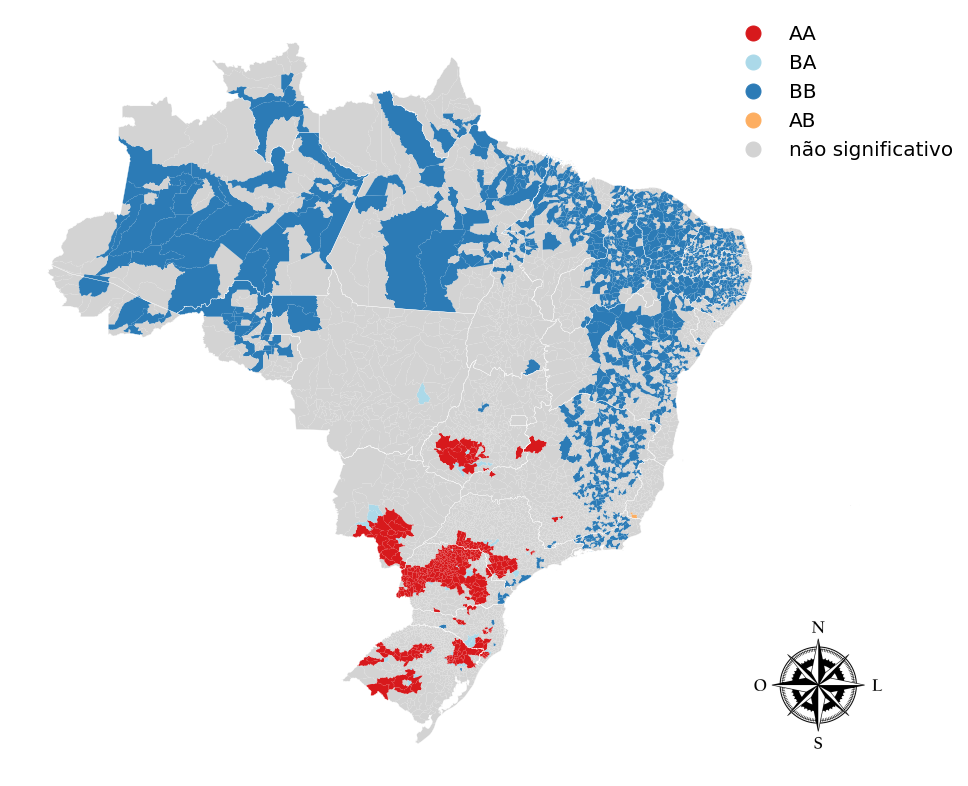
\includegraphics[width=0.6\textwidth]{img/map_lisa_ex.png}
%	\caption{Mapa de \textit{clusters LISA} para apólices contratadas de seguro rural}
%	\small \textsuperscript {Fonte: Elaboração própria}
%	\label{lisa_ex}
%\end{figure}


As duas estatísticas de autocorrelação espacial local apresentadas, o $G_i$ e o $I_i$, apresentam vantagens e desvantagens. Uma vantagem do $G_i$, em relação ao $I_i$, é a capacidade de estabelecer uma definição mais clara de \textit{clusters} com valores altos  (\textit{hot spots}) ou \textit{clusters} com valores baixos (\textit{cool spots}). Entretanto, o $I_i$ tem a vantagem de indicar uma associação espacial de valores dissimilares quando apresenta valores negativos. Ou seja, indica a presença de valores baixos da variável, circundados por valores altos ou valores altos rodeados por valores baixos. Estas observações, conhecidas como \textit{outliers} globais, não são captadas pelo $G_i$ \cite{darmofal06}.

\subsection{ESTATÍSTICA MULTIVARIADA}

%\subsubsection{Estatística multivariada}

A estatística multivariada é definida como um conjunto de métodos estatísticos que são empregados com o objetivo de analisar as variáveis como um todo, levando-se em conta, por exemplo, a sua estrutura de correlação. Considera-se que os dados são multivariados quando cada unidade amostral contém diversas variáveis aleatórias. Portanto, os métodos de estatística multivariada permitem a realização de uma avaliação muito mais abrangente do conjunto de dados, possibilitando a descoberta de padrões que, possivelmente, não seriam revelados ao se analisar cada variável individualmente \cite{mingoti10}.

Uma das formas de se classificar os métodos multivariados é proposta por Hair et al. (2009). Segundo a classificação dos autores, os métodos multivariados podem ser divididos como métodos de dependência e interdependência ou, \textit{supervised learning} e \textit{unsupervised learning}. Se for possível identificar variáveis com uma estrutura de dependência aconselha-se o uso de técnicas de dependência, tais como regressão múltipla, regressão logística ou análise discriminante. No entanto, se não houver uma distinção entre quais variáveis são dependentes e independentes, aconselha-se que o uso de técnicas de interdependência como análise fatorial e análise de agrupamento. 

Os dados multivariados são representados através de matrizes. Por exemplo, uma amostra aleatória que contenha $n$ observações contendo valores de $p$ variáveis observadas dá origem a uma matriz de dados $X$ com dimensão $n$ (linhas) por $p$ (colunas):

\begin{align}\label{X}
X_{n \times p} =
\left[
\begin{array}{cccc}
X_{11} & X_{12} & \dots & X_{1p} \\
X_{21} & X_{22} & \dots & X_{2p} \\
\vdots & \vdots & \ddots & \vdots \\
X_{n1} & X_{n2} & \dots & X_{np}\\
\end{array}
\right],
\end{align}

\noindent em que cada observação é representada por uma linha da matriz de dados $X$, sendo um vetor com $p$ variáveis, e cada variável é representada por uma coluna de $X$, sendo um vetor com $n$ elementos, as observações \cite{everitt11}.

A exposição de dados multivariados através de uma matriz como exposta na definição (\ref{X}) pode não ser muito informativa, principalmente se as dimensões $n$ e $p$ foram grandes. Dessa forma, faz-se necessário a utilização de medidas resumo dos dados amostrais, calculando-se a média, mediana, desvio padrão etc. de forma a sintetizar as informações dos dados da amostra \cite{ferreira11}.  

No caso multivariado, a média amostral, muito utilizada como uma medida de tendência central, torna-se o vetor de médias amostral de dimensão $p \times 1$, onde cada elemento $\bar{X}_{i}$, com $i = 1,2,\cdots,p $, é a média de uma variável:

\begin{align*}
	\boldsymbol{\bar{X}} = \left[
	\begin{array}{c}
		\bar{X}_1\\
		\bar{X}_2\\
		\vdots\\
		\bar{X}_p\\
	\end{array}
	\right].
\end{align*}

No caso multivariado,  utiliza-se, como medida de dispersão dos dados, no lugar da variância amostral, a matriz de covariâncias amostral $\boldsymbol{S}$ de dimensão $p \times p$. Esta matriz apresenta, em sua diagonal principal, as variâncias de cada uma das $p$ variáveis, e os elementos fora da diagonal principal são as covariâncias entre as variáveis. A matriz de covariâncias amostral é, portanto, simétrica, ou seja,  $S_{ij}$ $=$ $S_{ji}$.


\begin{align*}
	\boldsymbol{S} =
	\left[
	\begin{array}{cccc}
		S_{11} & S_{12} & \dots & S_{1p} \\
		S_{21} & S_{22} & \dots & S_{2p} \\
		\vdots & \vdots & \ddots & \vdots \\
		S_{p1} & S_{p2} & \dots & S_{pp} \\
	\end{array}
	\right].
\end{align*}        

Do mesmo modo, a correlação pode ser utilizada como uma medida de associação entre duas variáveis. Os possíveis valores do coeficiente de correlação se encontram no intervalo entre $-1$ e $1$. Valores próximos de $1$ apontam para o fato de  que as variáveis estão correlacionadas de forma positiva, ou seja, grandes valores de uma estão associados a grandes valores da outra. Por sua vez, valores próximos de $-1$ indicam que as variáveis estão correlacionadas de forma negativa, o que sugere que grandes valores de uma estão associados a pequenos valores da outra. A matriz de correlações amostral é dada por 

\begin{align*}
	\boldsymbol{R} =
	\left[
	\begin{array}{cccc}
		1      & r_{12} & \dots  & r_{1p} \\
		r_{21} & 1 & \dots  & r_{2p} \\
		\vdots & \vdots & \ddots & \vdots \\
		r_{p1} & r_{p2} & \dots  & 1\\
	\end{array}
	\right].
\end{align*}        

\noindent em que $r_{ij} = \frac{S_{ij}}{\sqrt{S_{ii} S_{jj}}}$ \cite{ferreira11}.  

\vspace{0.15cm} % só pra dar um espacinho :)

Para mais, outras estatísticas descritivas, como a matriz de somas de quadrados e produtos e a matriz de correlações, podem ser consideradas, dependendo do objetivo da pesquisa \cite{ferreira11}.

As técnicas de estatística multivariada podem ser classificadas em duas categorias, as técnicas exploratórias e as técnicas de inferência estatística. A primeira categoria compreende as técnicas que não dependem do conhecimento da forma matemática da distribuição de probabilidade que gerou a amostra de dados. O uso dessas técnicas permite a identificação de padrões em dados multivariados, o que faz com que estas técnicas possuam considerável apelo prático. É possível citar como exemplos de técnicas exploratórias análise de componentes principais, análise fatorial exploratória, análise de agrupamento. Em contraste, a categoria de técnicas de de inferência estatística têm como objetivo a estimação de parâmetros, testes de hipóteses, análise de regressão multivariada etc.  Dessa forma, as técnicas de inferência fazem uso da amostra para realizar inferências sobre a população de onde essa amostra foi extraída \cite{mingoti10}.

\subsection{ANÁLISE DE AGRUPAMENTO}

Também conhecida como classificação ou \textit{cluster analysis}, a análise de agrupamento é uma técnica exploratória que tem como objetivo encontrar partições (ou grupos) dos elementos de uma amostra. Os grupos são obtidos de maneira que as observações de um mesmo grupo sejam similares entre si em relação às variáveis analisadas e que as observações de grupos diferentes sejam heterogêneas em relação a essas mesmas variáveis \cite{mingoti10}.

Vários métodos, cujo objetivo é encontrar grupos de observações homogêneas, são considerados como ``análise de agrupamento''. Estes métodos procuram dar um tratamento matemático para o que os seres humanos são capazes de fazer de forma relativamente eficiente em duas ou três dimensões, por meio de diagramas de dispersão, por exemplo \cite{everitt11}. 

% Na análise de agrupamento, grupos são identificados pela avaliação das distâncias entre os pontos \cite{everitt11}. A título de ilustração, considere um conjunto de dados simulados em que há $n=300$ observações e duas variáveis aleatórias contínuas $p=2$. O objetivo é agrupar os dados em relação às duas variáveis. O diagrama de dispersão obtido se encontra no Gráfico \ref{fake_cluster} e é possível identificar $4$ agrupamentos, apenas pela análise visual. Se houvesse mais uma variável e, consequentemente mais uma dimensão, ainda seria possível imaginar um gráfico com os pontos. Porém, com mais de três dimensões a visualização dos dados torna-se mais complexa (BARTHOLOMEW et al., 2008).

%\begin{figure}[h!]
%	\centering
%	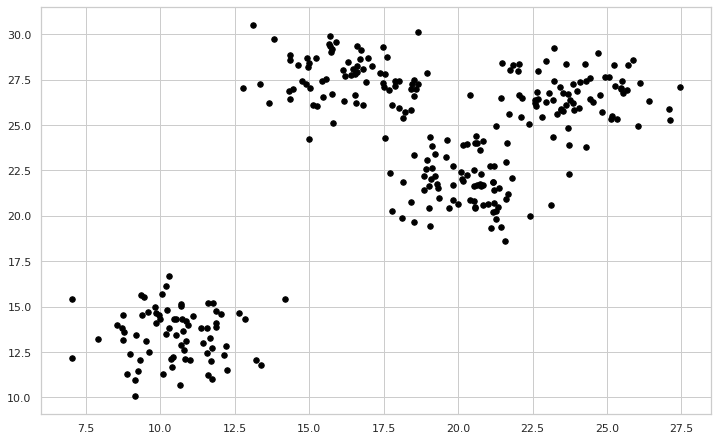
\includegraphics[width=0.6\textwidth]{img/fake_cluster.png}
%	\caption{Diagrama de dispersão de dados fictícios.}
%	\small \textsuperscript {Fonte: Elaboração própria com dados simulados}
%	\label{fake_cluster}
%\end{figure}

Existem duas possibilidades com relação aos objetivos dos métodos de agrupamento. A primeira delas é  agrupar as $n$ observações em um número desconhecido de grupos. Também há a possibilidade de classificar as observações em um conjunto predefinido de grupos. No primeiro caso, a análise de agrupamento deve ser utilizada, no segundo caso, a análise discriminante deve ser empregada. É importante ressaltar que, na análise de agrupamento, geralmente, o número de grupos não é conhecido a princípio e encontrar o melhor agrupamento não é considerado uma tarefa simples \cite{ferreira11}. 
Segundo Bartholomew et al. (2008), existem duas etapas fundamentais em qualquer processo de agrupamento. A primeira etapa consiste em obter as distâncias entre todos os pares de pontos para construção da matriz de distâncias. A segunda etapa compreende o desenvolvimento de um algoritmo para formação de grupos baseados nessas distâncias. 

As distâncias são definidas segundo medidas de similaridade ou dissimilaridade. As medidas de dissimilaridade correspondem às distâncias, ao passo que as de similaridades complementam as distâncias, assim, quanto maior a medida de similaridade entre dois objetos mais próximos eles serão \cite{ferreira11}. Algumas considerações a respeito de medidas de distâncias que podem ser utilizadas na análise de agrupamento serão apresentadas na próxima seção.

\subsubsection{Distâncias} 

A utilização de um algoritmo de agrupamento implica que se estabeleça, previamente, uma medida de distância. Há diversas medidas de similaridade ou dissimilaridade entre pares de observações. Entre as medidas de dissimilaridade mais comuns estão: a distância euclidiana, distância euclidiana padronizada, Manhattan, Mahalanobis, etc. É necessário destacar que, no caso de medidas de dissimilaridade, quanto menores os seus valores, mais próximos ou similares são os objetos comparados. Além disso, a escolha da métrica de distância interfere diretamente no resultado final do agrupamento \cite{mingoti10, everitt11}.  

%A distância entre as observações $i$ e $j$ é paresentada na $i$-ésima linha e $j$-ésima coluna da matriz de distâncias. Por exemplo, se há $n = 4$ elementos na amostra, a matriz de distâncias terá dimensão $4$ $\times$ $4$ e será da forma

%\begin{align*}
%	\left[
%	\begin{array}{cccc}
%		- & d_{12} & d_{13} & d_{14}\\
%		d_{21} & - & d_{23} & d_{24}\\
%		d_{31} & d_{32} & - & d_{34}\\
%		d_{41} & d_{42} & d_{43} & -\\
%	\end{array}
%	\right],
%\end{align*}

%\noindent em que $d_{ij}$ é a distância entre os elementos $i$ e $j$. Geralmente, essa matriz é simétrica, ou seja, $d_{12}=d_{21}$, $d_{13}=d_{31}$, e assim por diante (BARTHOLOMEW et al., 2008).

Uma das métricas de distância mais elementar é a distância euclidiana, que pode ser expressa por 

\begin{align*}
d_{ij} = \sqrt{\sum_{k = 1}^{p}(X_{ik} - X_{jk})^2},
\end{align*}

\noindent em que $d_{ij}$ é a distância euclidiana entre os elementos $i$, com os valores $X_{i1}$, $X_{i2}$, $\dots$, $X_{ip}$, e $j$, com os valores $X_{j1}$, $X_{j2}$, $\dots$, $X_{jp}$.

A distância de Mahalanobis e a euclidiana padronizada são generalizações da distância euclidiana. Sendo assim, a distância generalizada entre dois elementos $X_{i\cdot}$ e $X_{j\cdot}$ pode ser definida como  


\begin{align}
	d_{ij} = (X_{i\cdot} - X_{j\cdot})^T A(X_{i\cdot} - X_{j\cdot}). 
\end{align}

A seleção da matriz $A$ determina a distância a ser calculada. No caso em que $A= I$ obtém-se a distâncias euclidiana, se $A= D^{-1}$ tem-se como resultado a distância euclidiana padronizada. Se $A= S^{-1}$, ou seja, a inversa da matriz de covariâncias dos dados, obtém-se a distância de Mahalanobis \cite{mingoti10}.

%Nesse último caso, o cálculo das distâncias leva em consideração as diferenças de variâncias e covariâncias entre as variáveis \cite{mingoti10}.A medida de Mahalanobis, portanto, considera que objetos que possuem a mesma direção das correlações entre as variáveis sejam considerados mais similares entre si do que objetos situados em direções opostas. Além disso, essa medida de distância produz agrupamentos compactos e convexos e elimina o efeito de domínio na classificação das variáveis de maior variabilidade \cite{ferreira11}.

Após a definição da medida de distância a ser utilizada, o passo seguinte da análise consiste em escolher um método de agrupamento. De acordo com Ferreira (2011), os métodos de agrupamento podem ser classificados em não hierárquicos ou hierárquicos (aglomerativos ou divisivos). Nos métodos hierárquicos divisivos, no início, há um único grupo com as $n$ observações e, ao final, haverá $n$ grupos, cada um com uma observação. Nos métodos não hierárquicos é necessário definir o número de grupos $(k)$ previamente de forma que seja possível atribuir as $n$ observações aos $k$ grupos da melhor maneira possível. No início do processo utiliza-se uma alocação arbitrária e, iterativamente, busca-se a alocação ótima. Nos métodos hierárquicos aglomerativos ocorre o processo contrário, o processo de agrupamento se inicia com $n$ grupos, cada um contendo uma observação, no final do método haverá um único grupo com todas as observações. A cada passo do processo iterativo, cada observação ou grupo é unido a outra observação ou grupo. A união se dá através de um critério de similaridade, os objetos mais próximos entre si são alocados para o mesmo grupo, até que, no final, todos estejam em um único grupo \cite{ferreira11}.

\subsubsection{Técnicas hierárquicas aglomerativas}

Ao se utilizar o método hierárquico aglomerativo, depois que uma fusão é realizada, ela não será mais desfeita. Assim, quando o método coloca dois elementos em um mesmo grupo, eles não mais aparecerão em grupos diferentes. Dessa forma, para se encontrar uma solução adequada com o número de agrupamentos ótimo, é necessário adotar algum critério de divisão \cite{everitt11}.

Para ilustrar as fusões ou divisões realizadas a cada passo do processo de agrupamento, utiliza-se o dendrograma. Este tipo de gráfico tem a capacidade de representar os agrupamentos obtidos a partir de métodos hierárquicos, aglomerativos ou divisivos \cite{everitt11}. 

Um dos métodos hierárquicos aglomerativos mais frequentemente utilizado é o método de \textit{Ward}, ou método da mínima variância. Este método se fundamenta na mudança de variação entre os grupos e também dentro dos grupos que são formados em cada passo do algoritmo. Assim, a cada passo de agrupamento é calculada a soma de quadrados dentro dos grupos. Esta soma é composta do quadrado da distância euclidiana de cada elemento amostral pertencente ao grupo em relação à seu respectivo vetor de médias. A soma de quadrados dentro do $i$-ésimo grupo é definida como:  

\begin{align*}
SQDG_i = \sum_{j=1}^{n_i}(X_{ij} - \bar{X}_{i})^2,
\end{align*}
sendo $n_i$ o número de elementos no grupo $i$, $X_{ij}$ o vetor de observações do $j$-ésimo elemento amostral pertencente ao $i$-ésimo agrupamento e $\bar{X}_{i}$ o centróide do $i$-ésimo agrupamento, representando a soma de quadrados correspondente a tal grupo.

A distância entre dois grupos quaisquer, $G_i$ e $G_l$, é definida como:

\begin{align}\label{dist_g}
d_{ G_i,G_l} = \left(\dfrac{n_l n_i}{n_l + n_i}\right)(X_{ij} - \bar{X}_{i})^2.		
\end{align}

Em cada iteração do algoritmo, os dois grupos que minimizam a distância em (\ref{dist_g}) são combinados. Este método geralmente produz agrupamentos com aproximadamente o mesmo número de elementos em cada grupo e é adequado apenas para variáveis quantitativas por se baseado na comparação do vetor de médias amostral \cite{mingoti10}. 

\subsubsection{Técnica não hierárquica: \textit{K}-médias}

Outro algoritmo de agrupamento é conhecido como método das $k$-médias (ou \textit{k-means}). Este método busca por uma partição das $n$ observações em $k$ agrupamentos ($G_1$, $G_2$, $\cdots$, $G_k$), em que $G_i$ indica o conjunto de observações que pertence ao $i$-ésimo grupo e $k$ é dado por algum critério numérico de minimização. A implementação mais utilizada do método das $k$-médias tenta encontrar a partição dos $n$ elementos em $k$ grupos que minimize a soma de quadrados dentro dos grupos ($SQDG$) em relação a todas as variáveis. Esse critério pode ser escrito como 

\begin{align*}
SQDG = \sum_{j=1}^{p}\sum_{l=1}^{k}\sum_{i \in G_l}(X_{ij} - \bar{X}_{j}^{(l)})^2,
\end{align*}
em que $\bar{X}_{j}^{(l)} = \displaystyle\frac{1}{n_i}\sum_{i \in G_l}X_{ij}$ é a média dos indivíduos no grupo $G_l$ em relação à variável $j$ \cite{everitt11}.

Apesar de o problema parecer relativamente simples, ele não é tão elementar. A tarefa de selecionar a partição com a menor soma de quadrados dentro dos grupos se torna complexa pois o número de possíveis partições torna-se muito grande mesmo com um tamanho amostral não tão grande. Por exemplo, para $n = 100$ e $k=5$, o número de partições é da ordem de $10^{68}$. Este fato induziu o desenvolvimento de algoritmos que, embora não garantam encontrar a solução ótima, levam a soluções igualmente aceitáveis.

\subsubsection{Número de grupos}\label{n_grupos}

Independentemente do algoritmo utilizado, em aplicações de métodos de agrupamento, é necessário que se defina o número adequado de grupos. Isso se deve ao fato de que essa é a última etapa nos métodos de agrupamento hierárquicos aglomerativos e a etapa inicial nos agrupamentos não hierárquicos. 

Como exposto, nas técnicas hierárquicas aglomerativas, a cada passo, o algoritmo reúne duas observações ou grupos e ao final, um único grupo com as $k$ observações é obtido. Dessa forma, é necessário estabelecer uma regra de corte para que o número ideal de grupos seja escolhido. No caso de métodos não hierárquicos, como o das $k$-médias, por definição, o número de grupos seja escolhido a priori \cite{mingoti10}.

Alguns autores indicam a aplicação de uma combinação dos métodos hierárquicos e das $k$-médias. Nessa abordagem, primeiramente uma técnica hierárquica é aplicada para identificar o número de grupos e, em seguida, é aplicado o método das $k$-médias para classificar as observações \cite{hair09, mingoti10}. No entanto, em face a esta profusão de possíveis abordagens e, por não haver um critério adequado em todas as situações, é razoável levar em conta considerações de ordem práticas. Em algumas situações, é possível haver alguma informação a priori ou uma teoria que sugira uma estrutura nos dados. Ademais, a interpretabilidade e o significado prático e útil dos resultados deve ser o principal direcionador da escolha do número de grupos \cite{everitt11}.

%\newpage
\section{\textbf{MATERIAL E MÉTODOS}}\label{metodologia}

O objetivo desta seção é apresentar os dados utilizados no trabalho, quais as variáveis selecionadas, assim como descrever a metodologia usada na presente análise.

\subsection{Dados}
    
% Quais os dados 
Este trabalho utiliza dados referentes a apólices de seguro rural dos municípios brasileiros no ano de 2019. Os dados sobre seguro rural estão disponíveis no endereço eletrônico do Ministério da Agricultura, Pecuária e Abastecimento (MAPA). Também foram utilizados dados que contém atributos geográficos, como a posição e o formato, do território brasileiro. Esses dados estão disponíveis no endereço eletrônico do Instituto Brasileiro de Geografia e Estatística \cite{ibge20}. As variáveis utilizadas, bem como suas siglas e descrições, são apresentadas na Tabela \ref{variaveis}.
    
\begin{table}[h!]
    \begin{center}
    \caption{Descrição das variáveis utilizadas.} \label{variaveis}
    \footnotesize
    \begin{tabular}{ll}
        \hline 
        Variável & Sigla  \tabularnewline
        \hline 
        Total de apólices contratadas                  & TAC       \\ % ap\_contrat   
        Soma da importância segurada (R\$ milhão)      & SIS       \\ % t\_segurado   
        Soma dos prêmios (R\$ milhão)                  & SPR       \\ % soma\_premio  
        Total de subvenção (R\$ milhão)                & TSB       \\ % t\_subvencao  
        Soma das indenizações pagas (R\$ milhão)       & SIP       \\ % inde\_pagas   
        Taxa média aplicada às apólices                & TMA       \\ % tx\_media     
        Número de apólices indenizadas                 & NAI       \\ % ap\_indeniz   
        %\tabularnewline
        \hline 
        \vspace{0.1cm}
        \footnotesize{Fonte: Elaboração própria}
    \end{tabular}
    \end{center}
\end{table}
    
Como as variáveis estão em diferentes escalas e, com isto possuem diferentes variâncias, realizou-se a padronização das variáveis para que tais fatores não interferissem na análise. Tal padronização foi efetuada subtraindo-se de cada observação a média de sua respectiva variável e dividindo-se posteriormente pelo desvio padrão da variável.

\subsection{Metodologia}
    
Após a escolha das variáveis, foi realizada uma análise exploratória dos dados em que são apresentadas a distribuição espacial das variáveis, assim como a distribuição espacial das estatísticas de autocorrelação espacial \textit{I} de Moran e \textit{G} de Getis e Ord. Em seguida, é aplicado o procedimento, descrito a seguir, para descobrir e explorar padrões de agrupamento espacial com base na distribuição espacial de dados multivariados. 

O procedimento para a criação de agrupamentos com baseados medidas locais de autocorrelação espacial pode ser descrito da seguinte forma: 
    
\begin{enumerate}
    \item Dada uma matriz de pesos espaciais $W$, calcule para cada variável a estatística \textit{G} de Getis-Ord local. Seja $z(G_j(x_i))$ a estatística resultante de (\ref{g_getis_ord}) para a $j-$ésima variável no $i-$ésimo município; 
    \item Reúna os valores do passo anterior em uma matriz $Z$ de dimensão $(n \times p)$. Cada coluna de $Z$ expressa o padrão de autocorrelação local para uma variável, enquanto cada linha de $Z$ fornece o perfil de agrupamento em torno de cada unidade local; 
    \item Aplique o método de \textit{Ward} no conjunto $Z$ de novas variáveis para especificar o número de grupos a ser utilizado no método das $k$-médias;
	\item Aplique o algoritmo $k$-médias no conjunto $Z$. Esta etapa permite agrupar observações com base em seus perfis espaciais multivariados que contêm informações de localização e das variáveis.
\end{enumerate}     

O procedimento também foi empregado utilizando-se, como medida de autocorrelação espacial local, o \textit{I} de Moran local. 

Optou-se pelo método não hierárquico das $k$-médias para a etapa final, pois este método apresenta um desempenho superior aos métodos hierárquicos \cite{mingoti10}. %Além disso, com o uso dessa técnica, cada município foi alocado no grupo cujo vetor de médias amostral  era o mais semelhante ao vetor de valores observados para os respectivo município.
No entanto, como o método das $k$-médias impõe que seja inicialmente definido o número de grupos desejado, nessa abordagem, inicialmente foi utilizada uma técnica hierárquica para identificar este número\footnote{Alguns critérios para escolha do número de grupos foram apresentados na seção \ref{n_grupos}, dentre eles o uso de uma técnica hierárquica aglomerativa.}. Em seguida, o método das k-médias foi aplicado para classificar as observações. Nesse trabalho, optou-se pelo método de \textit{Ward} para especificar o número de grupos pretendido. Além de ser um método com desempenho superior aos demais,  ele é considerado indicado para dados quantitativos contínuos \cite{everitt11}. 

A definição do número de grupos da partição final da aplicação do método de \textit{Ward} foi realizada no final do processo de agrupamento, decidindo-se o ponto de corte no dendrograma. Dessa forma, foram utilizados os critérios da maior diferença no nível de fusão e da interpretabilidade. O primeiro critério faz referência à maior distância no dendrograma, que indica que o grupo pode se tornar menos homogêneo internamente com essa união \cite{everitt11}.  O segundo critério concerne à  solução que proporciona uma interpretação que corresponda aos objetivos da análise.  


\subsection{Recursos computacionais} 

Esse estudo foi realizado com a linguagem de programação \textit{Python} \cite{python17}, utilizando-se a interface \textit{Jupyter} \cite{jupyter17}, \cite{perez07} \cite{kluyver19}.
Além disso, as seguintes bibliotecas foram utilizadas: 
\textit{Pandas} \cite{mckinney10}, para a manipulação de dados,
\textit{NumPy} \cite{walt11}, que possibilita computação numérica com \textit{Python},
\textit{Matplotlib} \cite{hunter07} e \textit{Seaborn} \cite{waskom14}, que são bibliotecas para a criação de gráficos.
A análise de componentes principais foi realizada através da biblioteca \textit{sklearn} e as bibliotecas \textit{Geopandas} \cite{jordahl14} e \textit{PySAL} \cite{rey07} possibilitaram a análise espacial. Os códigos utilizados na análise estão disponíveis no \textit{GitHub} e os link estão no Apêndice \ref{codigos}. 

% RESULTADOS ========================================================================================================
%\newpage
\section{\textbf{RESULTADOS E DISCUSSÃO}} 

\subsection{Distribuição espacial}

A análise se inicia com a visualização da distribuição espacial das variáveis por meio dos mapas temáticos. Busca-se, através desses mapas, identificar visualmente se existem padrões na distribuição espacial das variáveis do seguro rural.

O primeiro grupo de mapas, apresentado na Figura \ref{mapa_variaveis}, exibe a distribuição espacial de cada uma das variáveis analisadas no ano de 2019. Pela análise da Figura 3, é possível constatar que a distribuição espacial das variáveis é bastante semelhante. Embora com distribuições espaciais muito similares entre si, as variáveis SIP (soma das indenizações pagas) e NAI (número de apólices indenizadas) diferem das demais variáveis. Este fato pode ser causado, entre outros motivos, pelo fato que estas variáveis se relacionam à ocorrência de sinistros. Além disso, é possível destacar que há indícios de concentrações espaciais de todas as variáveis nas regiões do Extremo Oeste Baiano (BA), Sudoeste de Mato Grosso do Sul, Sul Goiano (GO), na região Sudeste e no sul do Estado de São Paulo. 

\begin{figure}[h]
	\centering
	\caption{Distribuição espacial das variáveis de seguro rural.}
	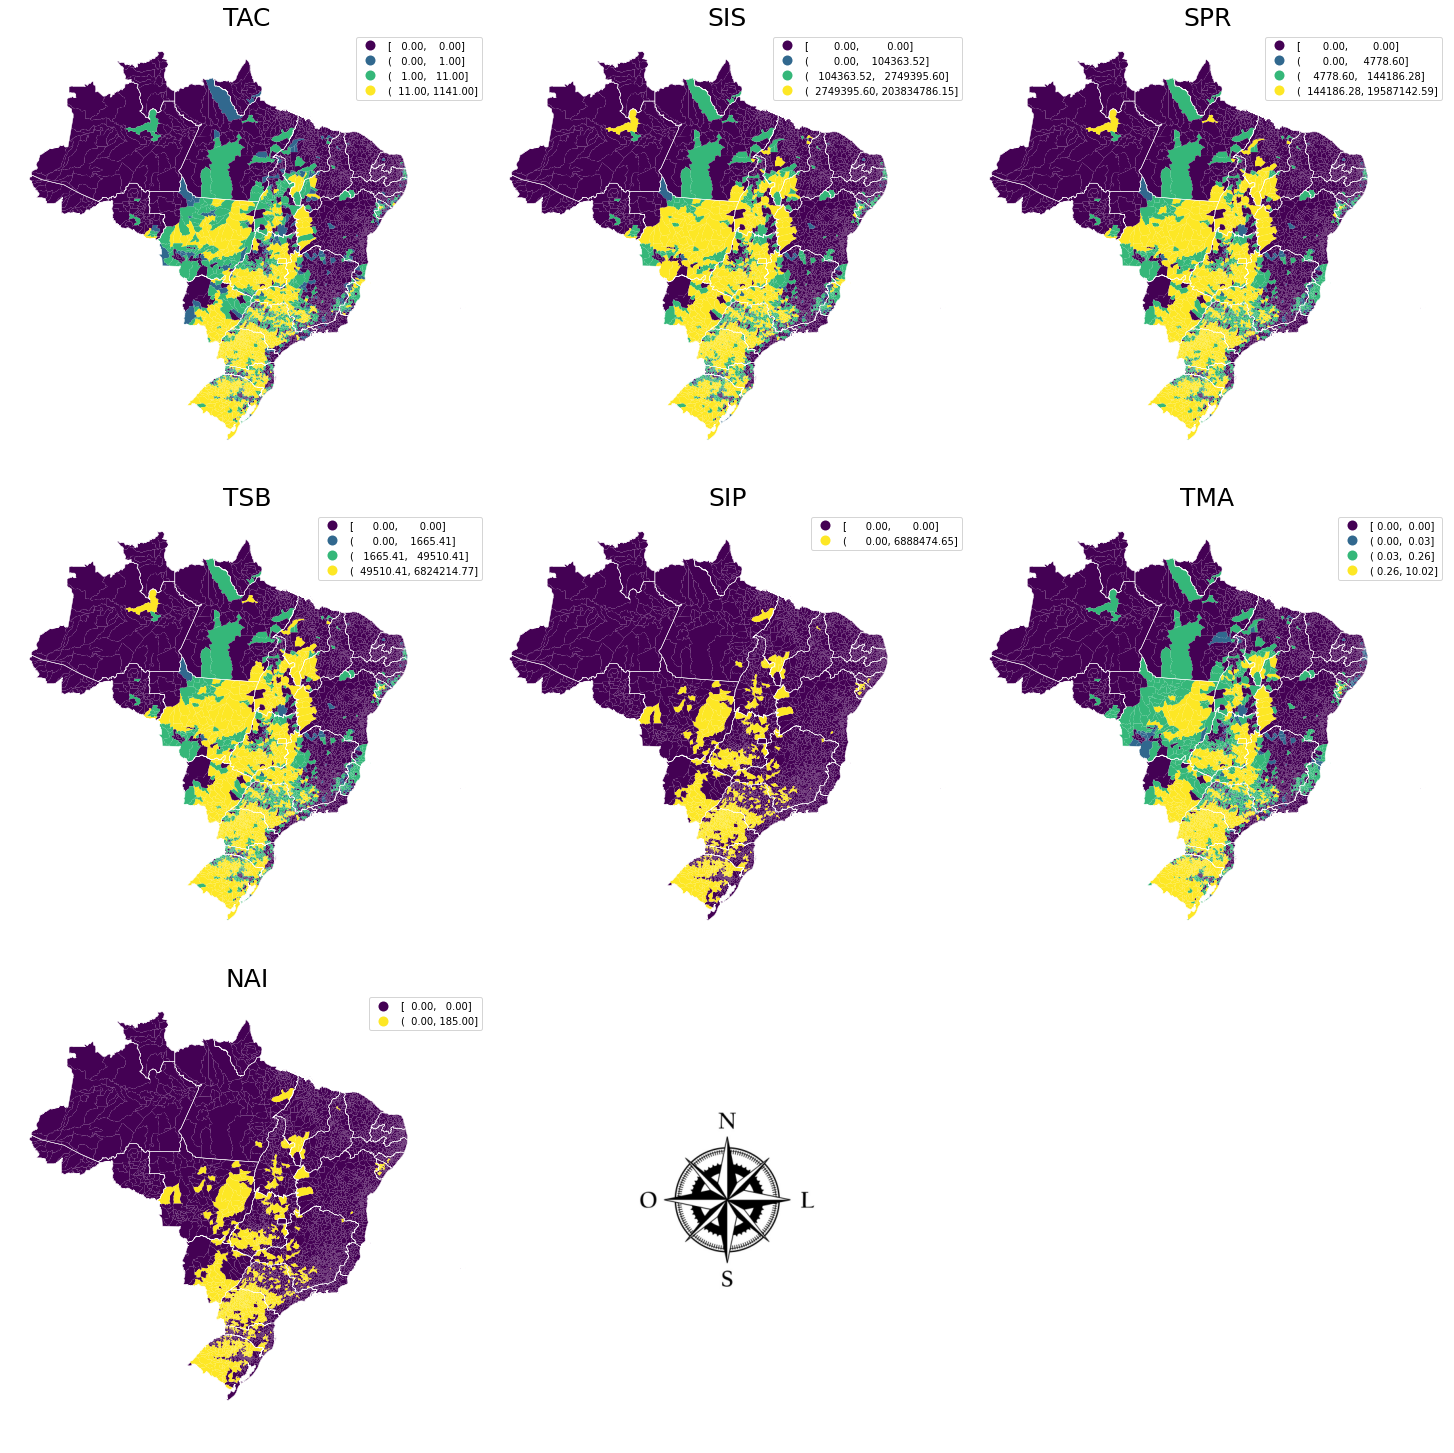
\includegraphics[width=0.9\textwidth]{img/map_variaveis.png}
	\noindent \small \textsuperscript{Fonte: Elaboração própria}
	\label{mapa_variaveis}
\end{figure}

A concentração regional do número de apólices, do valor de subvenção e, consequentemente, das demais variáveis do seguro rural acontece devido a motivos históricos e climáticos. De acordo com Santos e Silva (2017), isso ocorre pela presença de maiores riscos de intempéries nos estados da Região Sul, em São Paulo e Minas Gerais. Além disso, estados como Mato Grosso do Sul, Mato Grosso, Goiás, e a região formada pelos estados do Maranhão, Tocantins, Piauí e Bahia, mais recentemente, também têm aderido aos contratos de seguro rural devido a fatores climáticos \cite{santos17}. 

\subsection{Autocorrelação espacial}

O próximo passo da análise da distribuição espacial consistiu na construção dos mapas que representam a autocorrelação espacial local. Os mapas \textit{LISA} apresentam quatro grupos (Alto-Alto (AA), Baixo-Baixo (BB), Alto-Baixo (AB) e  Baixo-Alto (BA)) com características distintas de associação espacial estatisticamente significativas. Os mapas \textit{LISA} apresentados na Figura \ref{lisa_variaveis} apresentam os pontos que foram estatisticamente significativos no ano de $2019$. 

\begin{figure}[h]
	\centering
	\caption{Distribuição espacial do \textit{I} de Moran local para as variáveis de seguro rural.}
	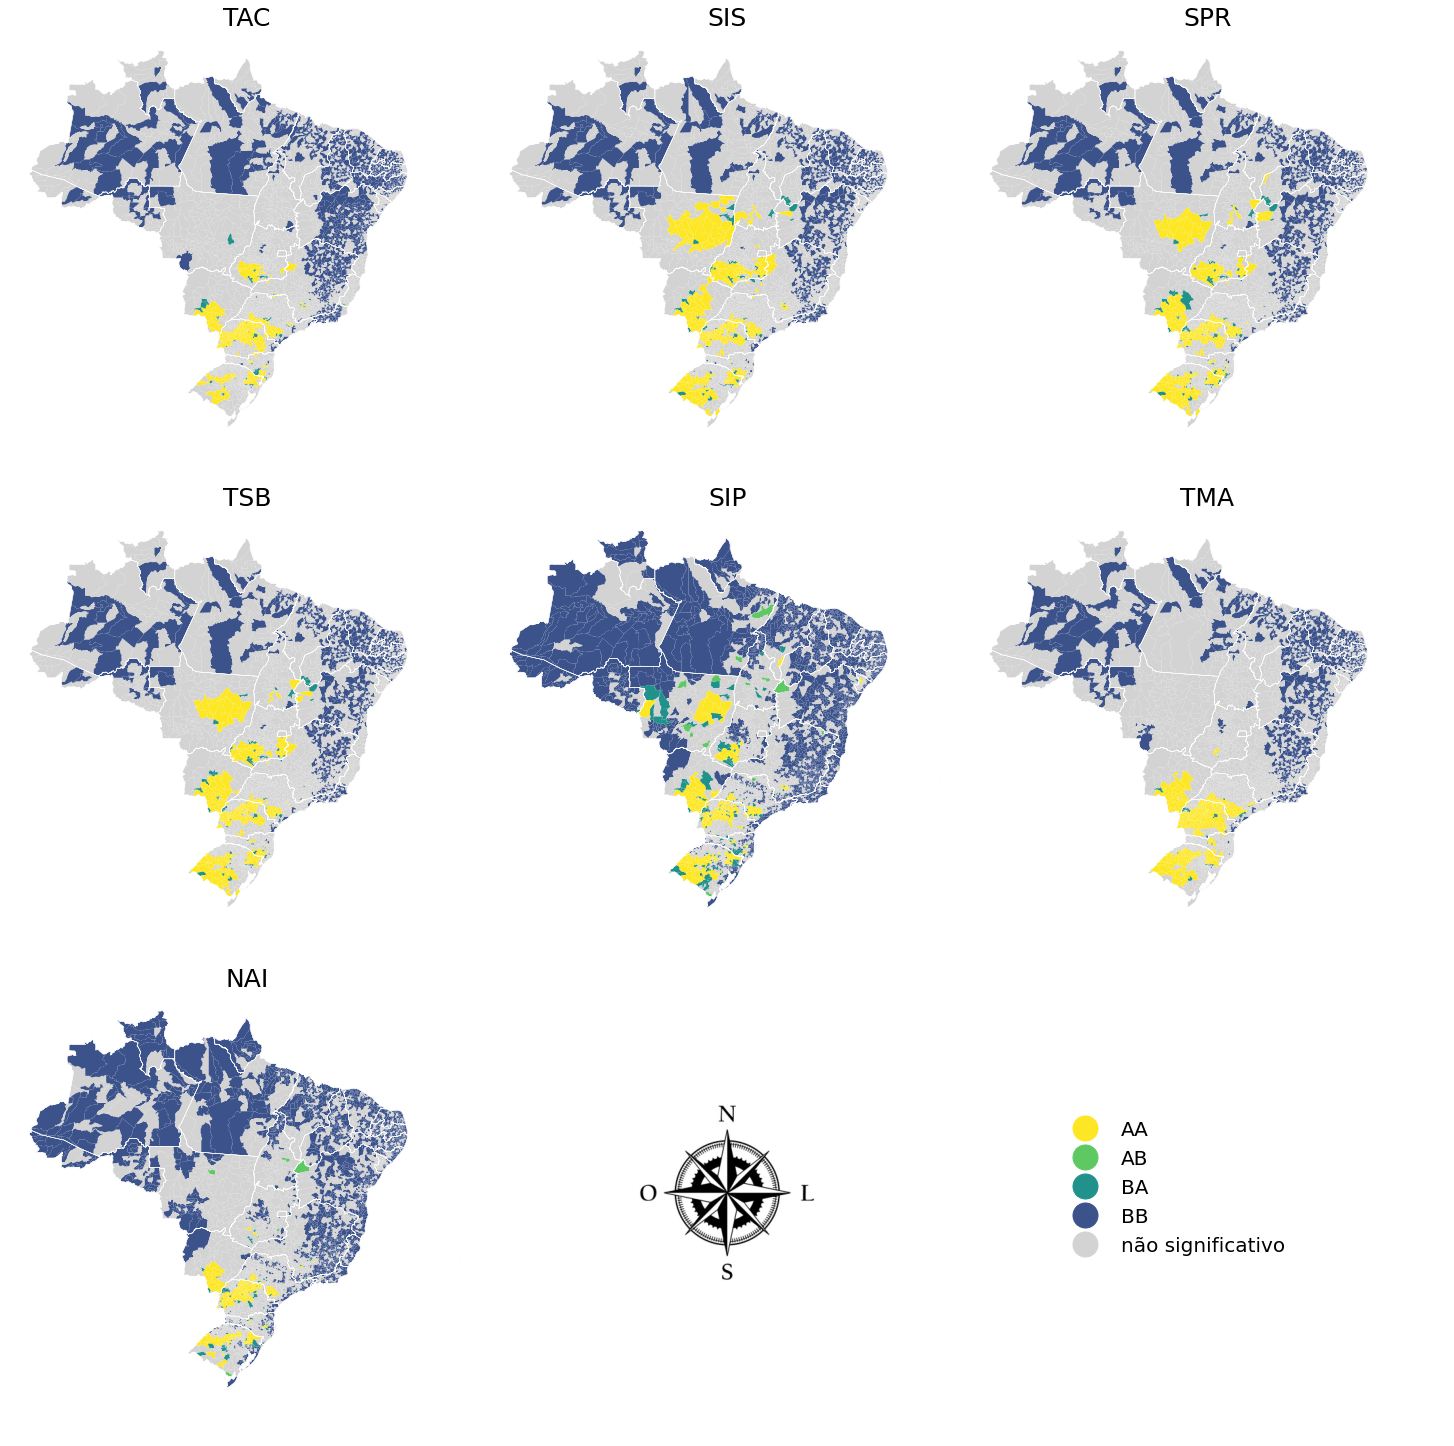
\includegraphics[width=0.9\textwidth]{img/map_i_moran_variaveis.png}
	\noindent \small \textsuperscript{Fonte: Elaboração própria}
	\label{lisa_variaveis}
\end{figure}

Na Figura \ref{lisa_variaveis} é possível identificar que a variável TAC apresenta concentrações de municípios do tipo AA nos estados de Goiás, Minas Gerais, Mato Grosso do Sul, São Paulo, Paraná, Santa Catarina e Rio Grande do Sul. A variável SIS, apresenta concentrações de municípios do tipo AA nos estados do Tocantins, Bahia, Mato Grosso, Mato Grosso do Sul, Goiás, Minas Gerais, São Paulo, Paraná, Santa Catarina e Rio Grande do Sul. Distribuições semelhantes também são observadas nas variáveis SPR, TSB e SIP, que também apresentam municípios do tipo AA e AB no estado do Piauí. Os municípios do tipo AA das variáveis TMA e NAI se concentram principalmente na região Sul do país e no sul do estado de São Paulo. Por sua vez, os agrupamentos de municípios do tipo BB se localizam, principalmente, nas regiões Norte e Nordeste. 

Os mapas apresentados na Figura \ref{g_variaveis} apresentam os agrupamentos das variáveis que foram estatisticamente significativos no ano de $2019$ considerando-se a estatística \textit{G} de Getis e Ord. Ou seja, apresenta agrupamentos localizados de concentração espacial (\textit{hot spots} e \textit{cool spots}).

\begin{figure}[h]
	\centering
	\caption{Distribuição espacial do \textit{G} de Getis e Ord local para as variáveis de seguro rural.}
	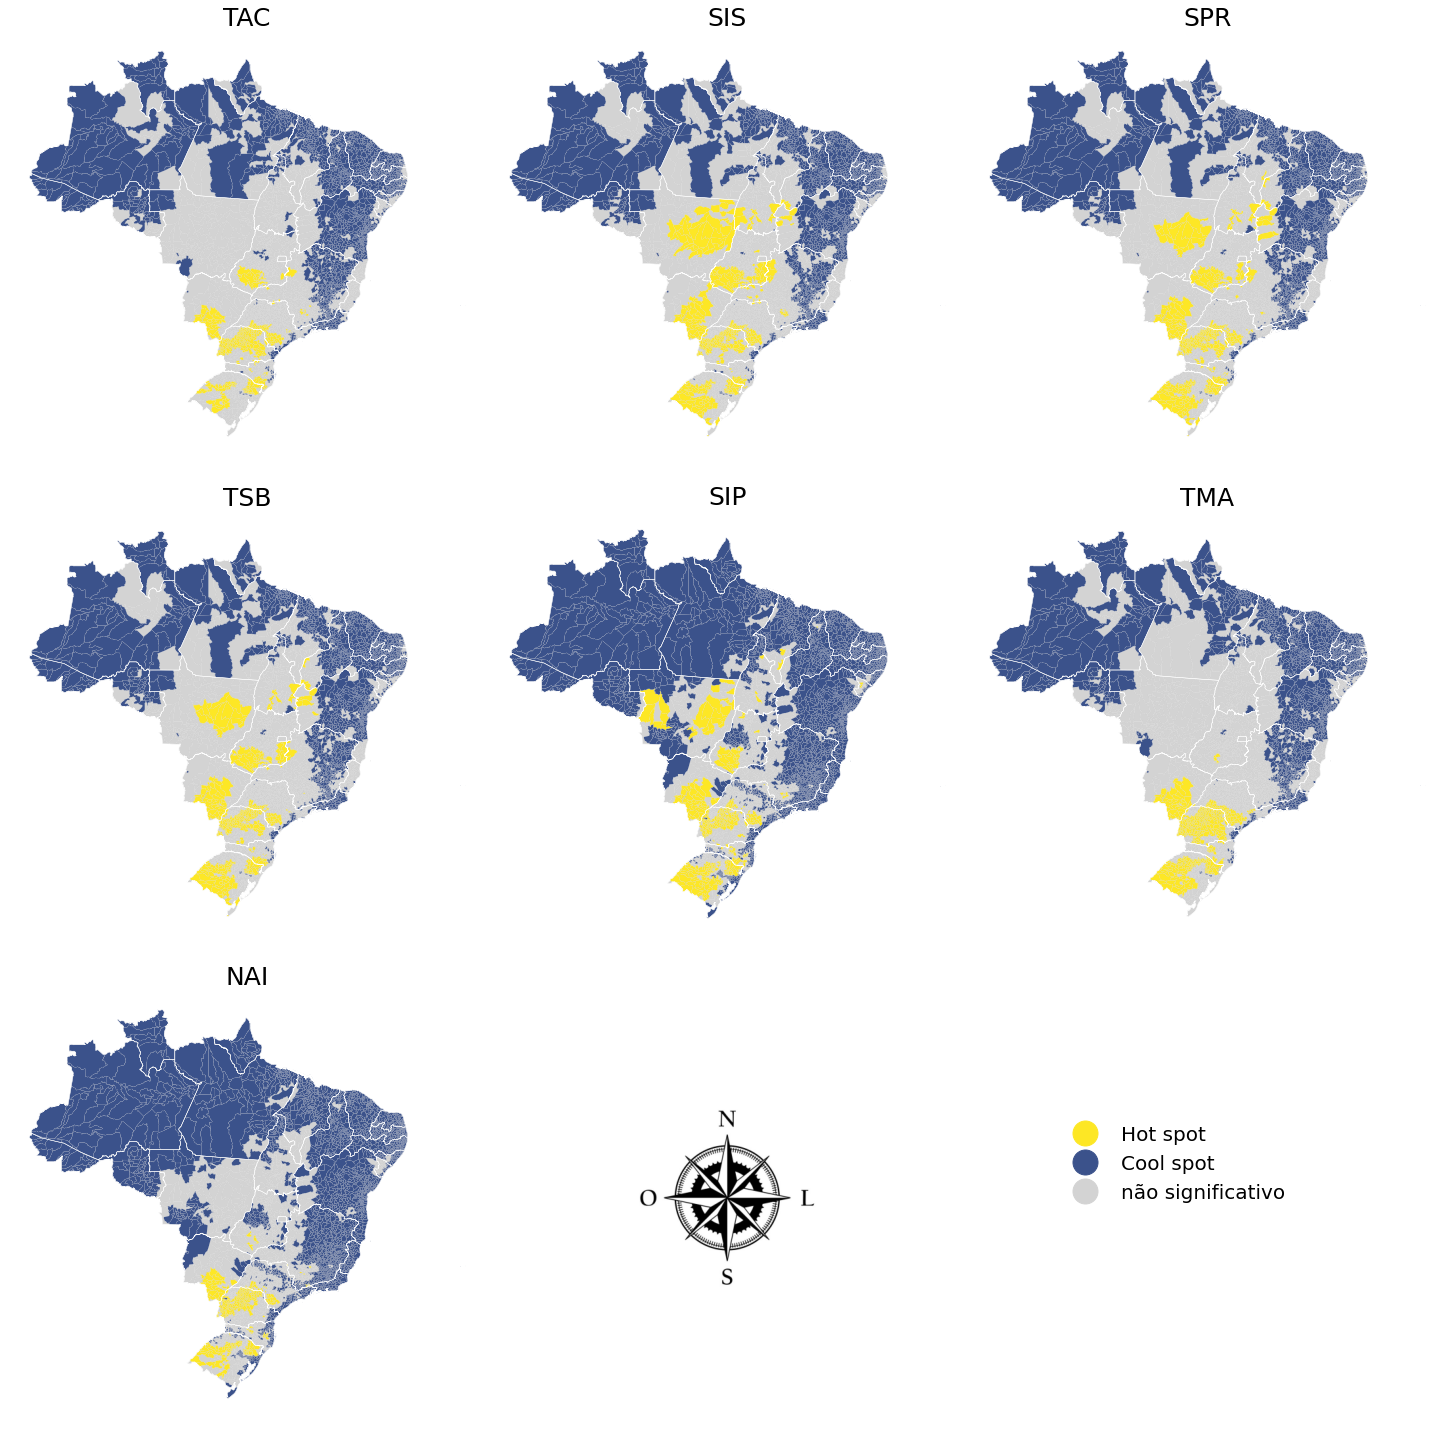
\includegraphics[width=0.9\textwidth]{img/map_getis_ord_variaveis.png}
	\noindent \small \textsuperscript{Fonte: Elaboração própria}
	\label{g_variaveis}
\end{figure}

É possível observar nos mapas da Figura \ref{g_variaveis} que os municípios do tipo \textit{hot spot}, ou seja, concentrações com valores altos da variável, se localizam, principalmente, nos estados da região Centro-Oeste, Sudeste e Sul. Mais especificamente, as variáveis TAI, TMA E NAI, apresentam concentrações de valores altos nos estados da região Sul, no sul do estado de São Paulo, em alguns municípios de Goiás e no estado do Mato Grosso do Sul. Os municípios do tipo \textit{hot spot} das variáveis SIS, SPR, TSB e SIP apresentam distribuição espacial semelhante àquela dos municípios do tipo AA. Essas variáveis apresentam concentrações de municípios do tipo \textit{hot spot} nos estados do Tocantins, Bahia, Mato Grosso, Mato Grosso do Sul, Goiás, Minas Gerais, São Paulo, Paraná, Santa Catarina e Rio Grande do Sul. 

\subsection{Identificação dos agrupamentos}

Em seguida, foi obtido o dendrograma da análise de agrupamento pelo método de \textit{Ward}, apresentado na Figura \ref{Dendrogramas}. O corte foi realizado na altura que classifica as observações em cinco grupos, para o caso do agrupamento realizado com o \textit{I} de Moran local (Figura \ref{Dendrogramas}\subref{Dendrogramas_a}), e quatro grupos, quando se considera o \textit{G} de Getis e Ord (Figura \ref{Dendrogramas}\subref{Dendrogramas_b}). Também foram examinadas as partições com dois grupos, no entanto, ao se considerar a interpretabilidade dos resultados, não foram encontradas evidências de que seriam mais adequadas. Dessa forma, o número predefinido de grupos usado para aplicação do método das $k$-médias foi cinco para os agrupamentos formados com o \textit{I} de Moran local, e quatro para os agrupamentos formados com o \textit{G} de Getis e Ord.

\begin{figure}[h]
	\caption{Dendrogramas}\label{Dendrogramas}
	\begin{center}
    	\subfigure[\textit{I} de Moran\label{Dendrogramas_a}]{
    	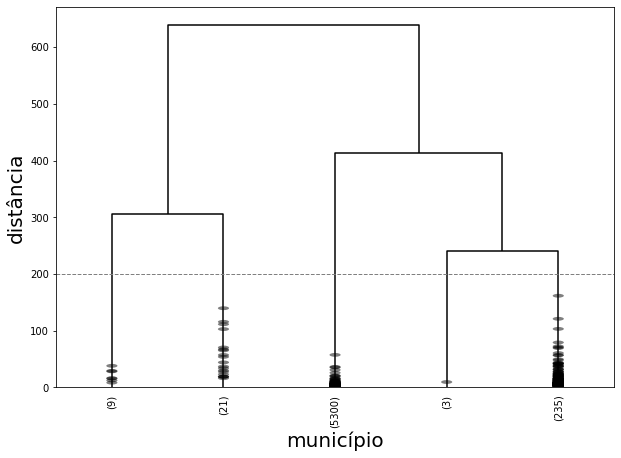
\includegraphics[width = 0.48\linewidth]{img/dendrograma_i_moran.png}}
    	\subfigure[\textit{G} de Getis e Ord\label{Dendrogramas_b}]{
    	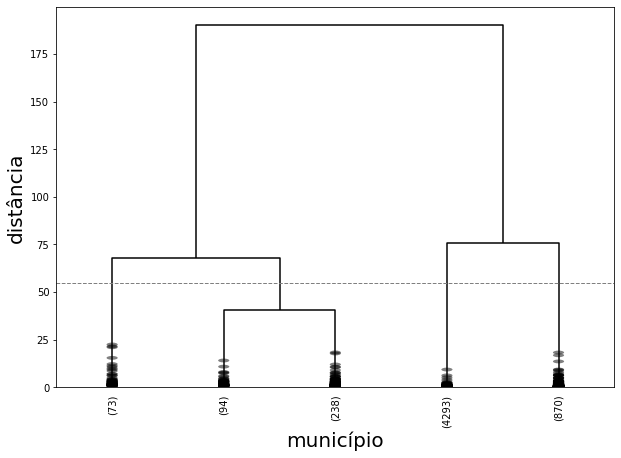
\includegraphics[width = 0.48\linewidth]{img/dendrograma_getis_ord.png}}
	\end{center}
	\noindent \small \textsuperscript{Fonte: Elaboração própria}
\end{figure}

O grupo de mapas apresentado na Figura \ref{cluster_ward} exibe a distribuição espacial dos agrupamentos formados pelo método de \textit{Ward} com \textit{I} de Moran (Figura \ref{cluster_ward}\subref{cluster_ward_a}) e \textit{G} de Getis e Ord (Figura \ref{cluster_ward}\subref{cluster_ward_b}). Pela análise da Figura \ref{cluster_ward}\subref{cluster_ward_a}, é possível observar que os municípios do grupo $1$ se localizam nos estados do Mato Grosso, Mato Grosso do Sul, Goiás, São Paulo, Paraná, Santa Catarina e Rio Grande do Sul. Os municípios do grupo $2$ se encontram no sul do estado de São Paulo, no estado do Paraná e no Nordeste Rio grandense. Por sua vez, os municípios pertencentes ao grupo $3$ localizam-se, principalmente, no Sudoeste do estado do Mato Grosso do Sul e Nordeste Rio grandense e região Serrana se Santa Catarina. Por fim, os municípios do  grupo $4$ se localizam na mesorregião Sudoeste Rio-Grandense no estado do Rio Grande do Sul. 

\begin{figure}[h]
	\caption{Agrupamentos formados pelo método de \textit{Ward} com \textit{I} de Moran e \textit{G} de Getis e Ord}\label{cluster_ward}
	\begin{center}
    	\subfigure[Grupos \textit{I} de Moran\label{cluster_ward_a}]{
    	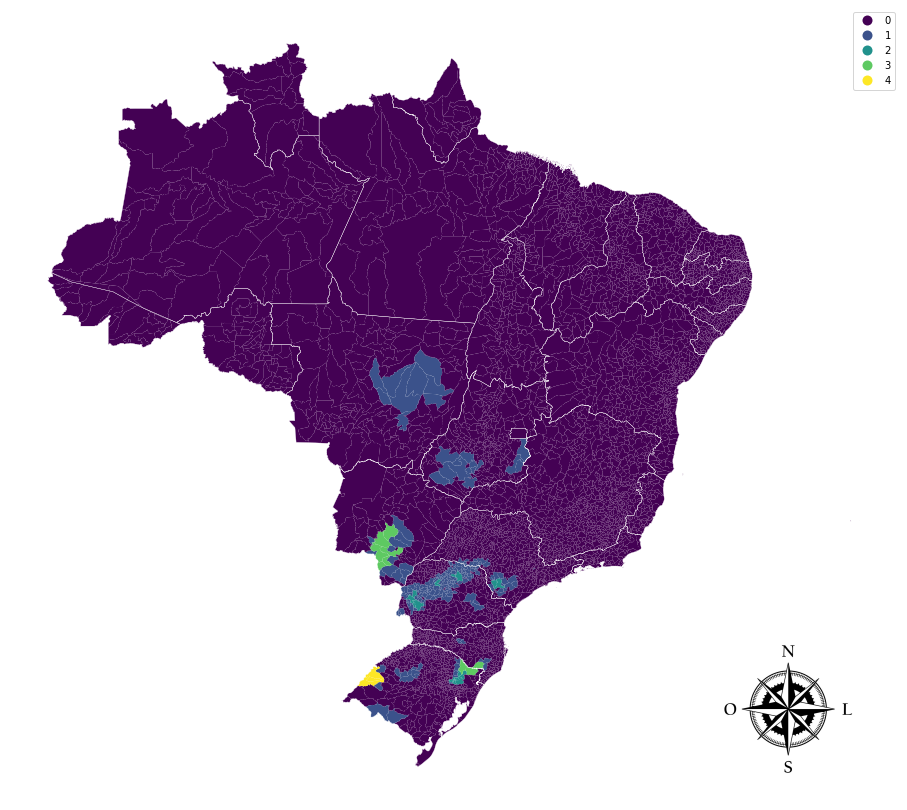
\includegraphics[width = 0.48\linewidth]{img/grupos_ward_i_moran.png}}
    	\subfigure[Grupos \textit{G} de Getis e Ord\label{cluster_ward_b}]{
    	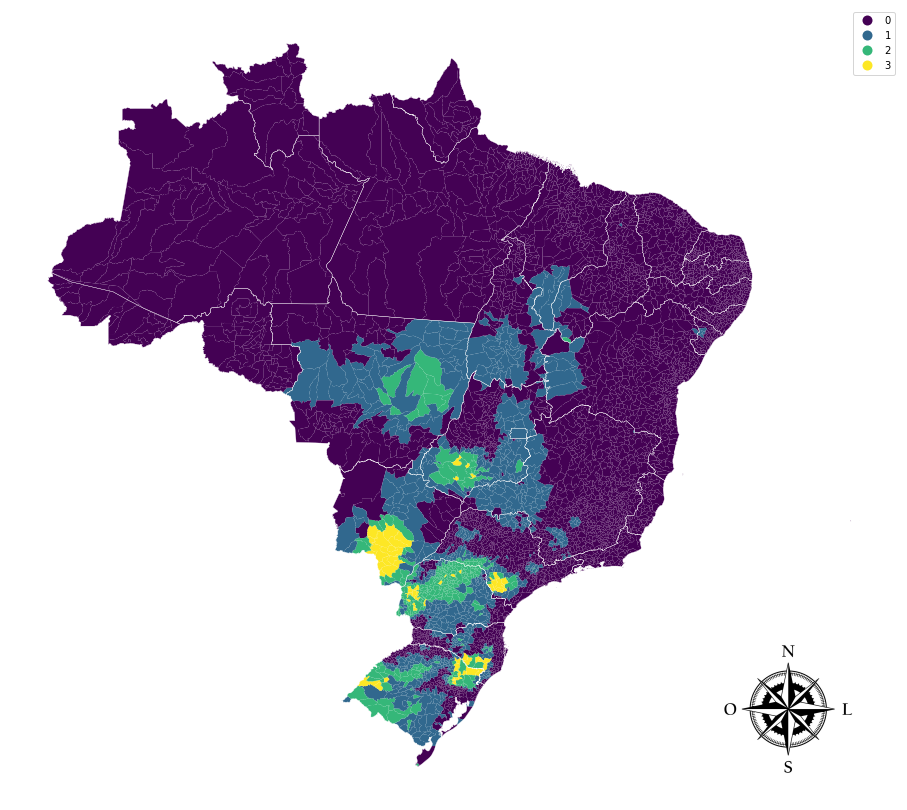
\includegraphics[width = 0.48\linewidth]{img/grupos_ward_getis_ord.png}}
	\end{center}
	\noindent \small \textsuperscript{Fonte: Elaboração própria}
\end{figure}

Nos agrupamentos formados utilizando a estatística \textit{G} de Getis e Ord (Figura \ref{cluster_ward}\subref{cluster_ward_b}) os municípios do grupo $1$ estão localizados nos estados do Maranhão, Piauí, Bahia e Sergipe na região Nordeste, nos estados da região Centro-Oeste, nos estados de Minas Gerais e São Paulo, no Sudeste, e nos estados da região Sul. Os municípios do grupo $2$ localizam-se, predominantemente, nas regiões Centro-Oeste e Sul, com exceção de alguns municípios localizados no Sul do estado de São Paulo. Por fim, os municípios pertencentes ao grupo 3 encontram-se no Sul Goiano, nas mesorregiões Sudoeste e Centro-Norte do Mato Grosso do Sul, na mesorregião de Itapetininga no estado de São Paulo, no Oeste Paranaense, na região Serrana de Santa Catarina e no Sudoeste e Nordeste Rio-Grandense.  

Para auxiliar na análise dos resultados a média das estatísticas $G_i$ e do \textit{I} de Moran nos grupos formados pelos métodos de \textit{Ward} e das  $k-$médias são apresentados nas tabelas \ref{mean_G} e \ref{mean_I}, respectivamente. A partir desses resultados, foi possível encontrar o perfil de autocorrelação espacial de cada agrupamento resultante.

\begin{table}[h]
    \caption{Média da estatística $G_i$ nos grupos formados pelos métodos de \textit{Ward} e das  $k-$médias} \label{mean_G}
    \footnotesize
    \vspace{0.05cm}
    \begin{tabularx}{\textwidth}{lRRRRRRRR}
        \hline \\[-1.9ex]	 
        Método de agrupamento & Grupos & \multicolumn{7}{c}{Variáveis}\\
        \cmidrule{3-9}
                      &   & TAC   & SIS   & SPR   & TSB   & SIP  & TMA   & NAI   \\
        \hline \\[-1.9ex]	 
                         & 0 & -0,25 & -0,25 & -0,24 & -0,24 & -0,19 & -0,31 & -0,20 \\
        \textit{Ward}    & 1 &  0,34 &  0,56 &  0,42 &  0,42 &  0,31 &  0,54 &  0,18 \\
                         & 2 &  2,19 &  1,82 &  1,80 &  1,81 &  1,57 &  2,63 &  2,04 \\
                         & 3 &  4,29 &  4,56 &  4,90 &  4,91 &  3,70 &  3,37 &  3,13 \\
        \hline \\[-1,9ex]	 
                         & 0 & -0,23 & -0,23 & -0,22 & -0,22 & -0,18 & -0,29 & -0,19 \\
        $k-$médias       & 1 &  0,47 &  0,73 &  0,57 &  0,57 &  0,40 &  0,72 &  0,27 \\
                         & 2 &  4,43 &  4,22 &  4,40 &  4,41 &  3,61 &  3,65 &  3,60 \\
                         & 3 &  2,14 &  1,74 &  1,81 &  1,81 &  1,59 &  2,65 &  1,98 \\
        \hline 
    \end{tabularx} 
    \footnotesize{Fonte: Elaboração própria.  }\\
\end{table}

Os grupos formados pelo método de \textit{Ward} apontam para uma caracterização de grupos em que o grupo $0$ é formado por concentrações do tipo \textit{cool spot}. Ou seja, o grupo $0$ é constituído por municípios com valores baixos de todas as variáveis. O grupo $1$ caracteriza-se por concentrações do tipo \textit{hot spot} com valores da estatística $G_i$ entre $0,56$  na variável SIS e $0,18$ na variável NAI. Por sua vez, o grupo 2 também é constituído de municípios classificados como \textit{hot spot} e o valor da estatística $G_i$ varia de $1,57$ na variável SIP a $2,36$ na variável TMA. Além disso, observa-se na tabela \ref{mean_G} que a utilização do método das $k-$médias apresenta uma divisão de grupos com características muito semelhantes àquela feita pelo método de \textit{Ward}. Ou seja, o grupo $0$ é o único constituído de municípios com característica de concentração de valores baixos das variáveis (\textit{cool spots}) e os demais grupos apresentam concentrações de valores altos das variáveis (\textit{hot spots}).

%Os gráficos apresentados na Figura \ref{sqdg} exibem a relação entre a soma de quadrados dentro dos grupos e o número de grupos na aplicação do método das $k$-médias. Na Figura \ref{sqdg}\subref{sqdg_a}, a soma de quadrados é obtida através do agrupamentos dos valores do \textit{I} de Moran local e na Figura \ref{sqdg}\subref{sqdg_b}, a soma de quadrados advém dos agrupamentos da estatística \textit{G} de Getis e Ord. 


%\begin{figure}[h!]
%	\caption{Soma de quadrados dentro dos grupos.}\label{sqdg}
%	\begin{center}
%    	\subfigure[\textit{I} de Moran\label{sqdg_a}]{
%    	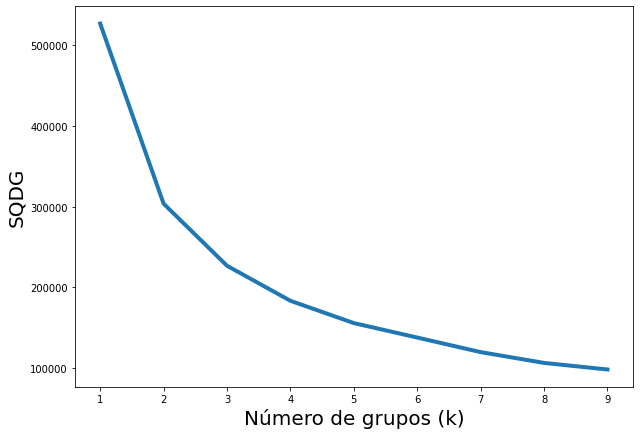
\includegraphics[width = 0.48\linewidth]{img/sqdg_i_moran.png}}
%    	\subfigure[\textit{G} de Getis e Ord\label{sqdg_b}]{
%    	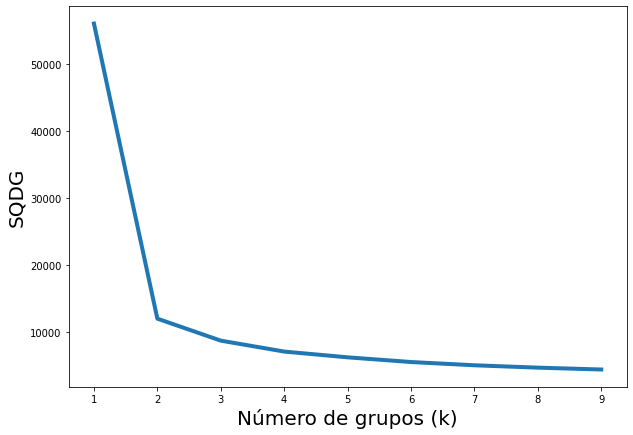
\includegraphics[width = 0.48\linewidth]{img/sqdg_getis_ord.png}}
%	\end{center}
%	\noindent Fonte: Elaboração própria
%\end{figure}


Os mapas apresentados na Figura \ref{cluster_kmedia} apresentam a distribuição espacial dos agrupamentos formados pelo método das $k-$médias com \textit{I} de Moran (Figura \ref{cluster_kmedia}\subref{cluster_kmedia_a}) e \textit{G} de Getis e Ord (Figura \ref{cluster_kmedia}\subref{cluster_kmedia_b}).  Pela análise da Figura \ref{cluster_kmedia}\subref{cluster_kmedia_a}, observa-se que os municípios do grupo $1$ localizam-se nos estados do Mato Grosso, Mato Grosso do Sul, Goiás, São Paulo, Paraná, Santa Catarina e Rio Grande do Sul. Por sua vez, os municípios pertencentes ao grupo $2$ se encontram no sul do estado se São Paulo, no estado do Paraná e no Nordeste Rio grandense. Já os municípios do grupo $3$ se localizam, principalmente, no Sudoeste do estado do Mato Grosso do Sul e Nordeste Rio grandense e região Serrana de Santa Catarina. Por último, os municípios pertencentes ao grupo $4$ localizam-se na mesorregião Sudoeste Rio-Grandense no estado do Rio Grande do Sul. 

\begin{figure}[h!]
	\caption{Agrupamentos formados pelo método das $k-$médias com \textit{I} de Moran e \textit{G} de Getis e Ord}\label{cluster_kmedia}
	\begin{center}
    	\subfigure[Grupos \textit{I} de Moran\label{cluster_kmedia_a}]{
    	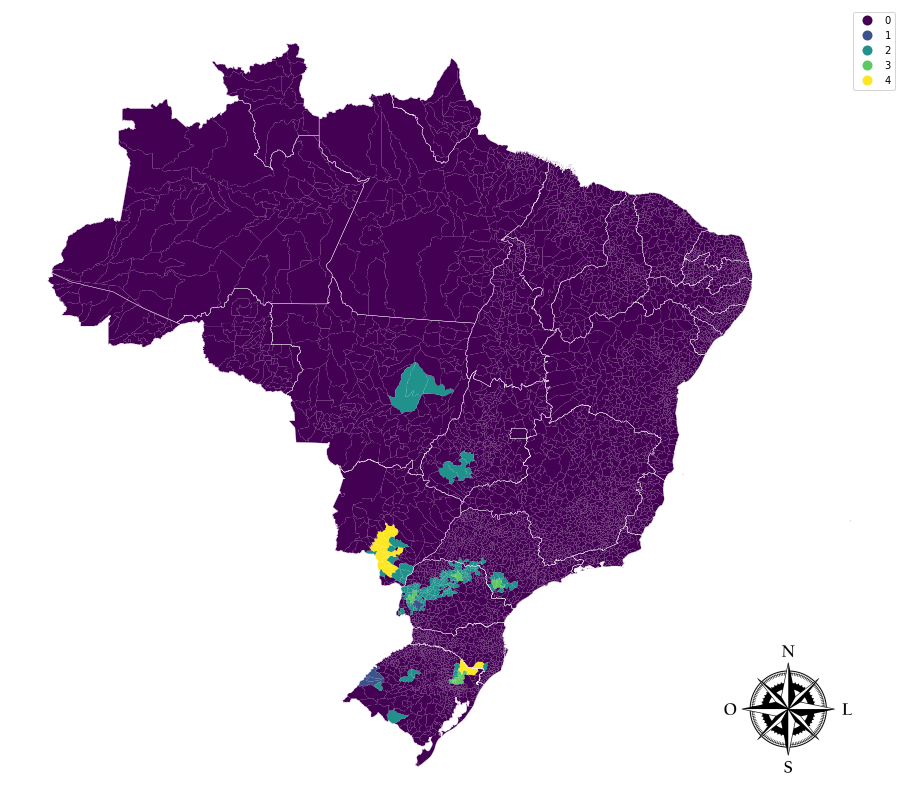
\includegraphics[width = 0.48\linewidth]{img/grupos_kmedias_i_moran.png}}
    	\subfigure[Grupos \textit{G} de Getis e Ord\label{cluster_kmedia_b}]{
    	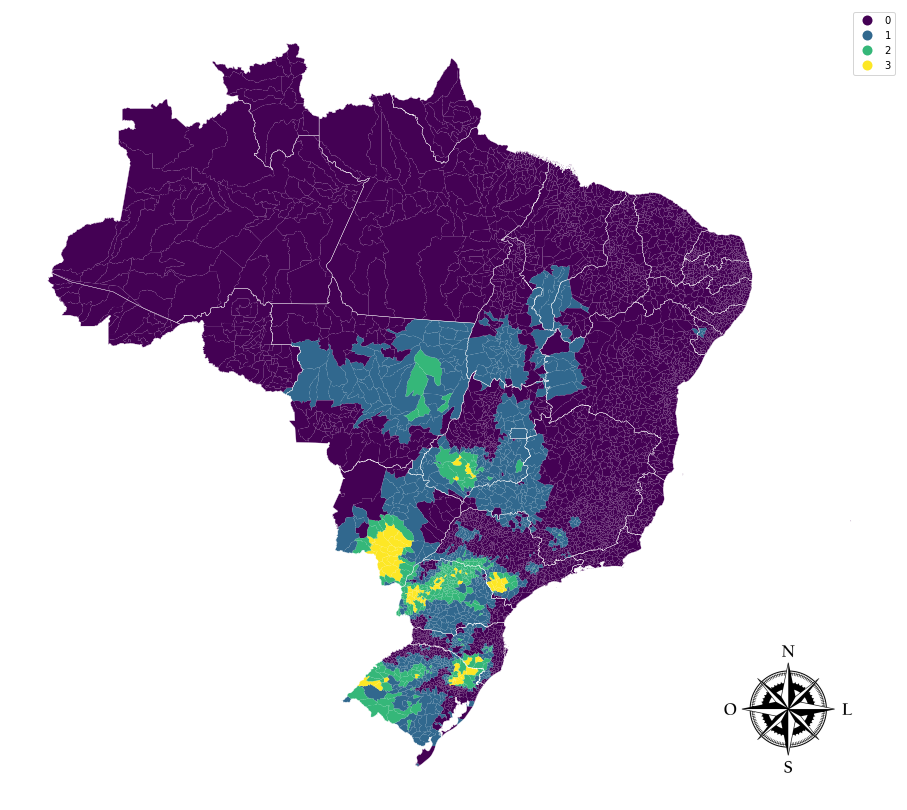
\includegraphics[width = 0.48\linewidth]{img/grupos_kmedias_getis_ord.png}}
	\end{center}
	\noindent \small \textsuperscript{Fonte: Elaboração própria}
\end{figure}

A Figura \ref{cluster_kmedia}\subref{cluster_kmedia_b} apresenta os agrupamentos formados utilizando a estatística \textit{G} de Getis e Ord. Observa-se que os municípios pertencentes ao grupo $1$ estão localizados nos estados do Maranhão, Piauí, Bahia e Sergipe na região Nordeste, nos estados da região Centro-Oeste, nos estados de Minas Gerais e São Paulo, no Sudeste, e nos estados da região Sul. Por sua vez, os municípios do grupo $2$ se localizam nas regiões Centro-Oeste e Sul, com exceção de alguns municípios localizados no Sul do estado de São Paulo. Por fim, os municípios classificados como pertencentes ao grupo $3$, encontram-se no Sul Goiano, nas mesorregiões Sudoeste e Centro-Norte do Mato Grosso do Sul, na mesorregião de Itapetininga no estado de São Paulo, no Oeste Paranaense, na região Serrana de Santa Catarina e no Sudoeste e Nordeste Rio-Grandense.

\begin{table}[h]
    \caption{Média da estatística \textit{I} de Moran nos grupos formados pelos métodos de \textit{Ward} e das  $k-$médias} \label{mean_I}
    \footnotesize
    \vspace{0.05cm}
    \begin{tabularx}{\textwidth}{lcRRRRRRR}
        \hline \\[-1.9ex]	 
        Método de agrupamento & Grupos & \multicolumn{7}{c}{Variáveis}\\
        \cmidrule{3-9}
                      &   & TAC   & SIS   & SPR   & TSB   & SIP  & TMA   & NAI   \\
        \hline \\[-1.9ex]	 
                      & 0 &   0,11 &   0,12 &   0,09 &   0,09 &   0,08 &   0,26 &   0,11 \\
                      & 1 &   7,50 &   6,18 &   5,43 &   5,48 &   3,91 &  11,15 &   5,68 \\
        \textit{Ward} & 2 &  55,71 &  21,25 &  23,71 &  23,66 &  16,12 &  25,49 &  43,24 \\
                      & 3 &  14,16 &  44,68 &  62,54 &  64,17 &  11,47 &   7,50 &   4,27 \\
                      & 4 &   1,33 &  10,35 &  15,23 &  13,95 & 101,29 &   6,81 &   5,06 \\
        \hline \\[-1,9ex]	 
                      & 0 &   0,14 &   0,17 &   0,13 &   0,13 &   0,09  &   0,32 &   0,12 \\
                      & 1 &   6,23 &   8,65 &  12,17 &  11,43 &  82,02  &  14,88 &  25,84 \\
        $k-$médias    & 2 &  10,29 &   7,06 &   6,39 &   6,46 &   5,15  &  13,60 &   8,27 \\
                      & 3 &  65,42 &  25,53 &  29,04 &  28,90 &  13,88  &  28,56 &  45,68 \\
                      & 4 &  13,62 &  43,16 &  59,62 &  61,16 &  13,41  &   7,54 &   4,45 \\
        \hline 
    \end{tabularx} 
    \footnotesize{Fonte: Elaboração própria.  }\\
\end{table}

       
É possível observar na Tabela \ref{mean_I} que o grupo $0$ é constituído por municípios com valores mais baixos da estatística \textit{I} de Moran local em ambos os métodos, $k-$médias e \textit{Ward}. O grupo $1$ é o segundo grupo com maiores valores do \textit{I} de Moran local. Os grupos $2$ e $3$ são os grupos com maiores valores de \textit{I} de Moran local. 

Diferentes razões podem considerados como determinantes da concentração do mercado de seguro rural em algumas regiões brasileiras. De acordo com Santos, Sousa e Alvarenga (2013), os principais fatores que devem ser considerados são: o pequeno número e as disparidades no porte das seguradoras que oferecem o seguro rural, dificuldades das instituições bancárias com operações no meio rural, levando a informações imprecisas e à elevação de riscos e preços, parcerias governamentais com operadores, como por exemplo, programas de crédito oficial operados pelo Banco do Brasil, que também é o controlador da maior seguradora agrícola,  o grau de oportunidade avaliado como pequeno pelas seguradoras, e por fim, o pequeno peso de parcerias e de avaliação das oportunidades envolvendo o segmento de corretagem.   

\newpage
\section{\textbf{CONSIDERAÇÕES FINAIS}} \label{secconsfinais}


O objetivo deste trabalho foi encontrar agrupamentos de municípios com características semelhantes em relação à adesão ao seguro rural no ano de $2019$. Os agrupamentos foram obtidos de forma a levar em consideração não apenas o valor das variáveis de seguro rural, mas também seu posicionamento geográfico. 

Os resultados da AEDE apontam que existe dependência espacial em todas as variáveis. Ou seja, existem padrões de associação espacial estatisticamente significativos. Também foi possível identificar a presença de \textit{clusters} espaciais significativos. Tal resultado é observado em todas as variáveis de seguro rural analisadas. 

Em geral, identificou-se que as maiores concentrações de apólices de seguro rural estão situadas nas regiões Sul, Centro-Oeste e Sudeste, no sul do Estado de São Paulo. Ou seja, municípios que possuem uma maior adesão ao seguro rural tendem a ser geografica mente próximos de municípios que também têm maior número de apólices de seguro rural contratadas. Além disso, ressalta-se que, embora exista uma concentração do número de apólices contratadas, número de apólices indenizadas, valores de subvenção, indenização e prêmio, atualmente há expansão da demanda por seguros agrícolas. 

Apesar de os dados indicarem uma concentração geográfica da adesão ao sistema de seguro rural no Brasil, é necessário levar em consideração outros sistemas, como o Proagro e o programa Garantia Safra. É necessário, ainda, ressaltar que a adesão dos produtores deve ocorrer como uma resposta à percepção do risco das atividades agropecuárias, ou seja, o seguro deve difundir-se com base na compreensão dos riscos e das vantagens de sua contratação. 

\newpage
	
\providecommand{\abntreprintinfo}[1]{%
 \citeonline{#1}}
\setlength{\labelsep}{0pt}\begin{thebibliography}{}
\providecommand{\abntrefinfo}[3]{}
\providecommand{\abntbstabout}[1]{}
\abntbstabout{v-1.9.6}

    \bibitem[almeida12]{almeida12}
    \abntrefinfo{almeida12}{ALMEIDA}{2012}
    {ALMEIDA, E. \textbf{Econometria Espacial Aplicada}. Campinas-SP: Alínea, 2012.}
    
    \bibitem[anselin95]{anselin95}
    \abntrefinfo{anselin95}{ANSELIN}{1995}
    {ANSELIN, Luc. Local indicators of spatial association -- LISA. \textbf{Geographical analysis}, v. 27, n. 2, p. 93-115, 1995.}
    
    \bibitem[barros12]{barros12}
    \abntrefinfo{barros12}{BARROS \textit{et al}}{2012}
    {BARROS, A. et al. Seguro Agrícola no Brasil: uma visão estratégica de sua importância para a economia brasileira. \textbf{MB Agro}, 2012.}
    
    \bibitem[brasil19]{brasil19} 
    \abntrefinfo{brasil19}{BRASIL}{2019a}
    {BRASIL. \textbf{Agropecuária Brasileira em Números}. Brasília, DF: Brasília: Ministério da Agricultura, Pecuária e Abastecimento (MAPA), 2019a }
    
    \bibitem[brasil19b]{brasil19b} 
    \abntrefinfo{brasil19b}{BRASIL}{2019b}
    {BRASIL. \textbf{Programa de Subvenção ao Prêmio do Seguro Rural: Relatório de Resultado 2018}. Brasília, DF: Brasília: Ministério da Agricultura, Pecuária e Abastecimento (MAPA), 2019b.}
    
    \bibitem[brasil21]{brasil21} 
    \abntrefinfo{brasil21}{BRASIL}{2021a}
    {BRASIL. \textbf{Programa de Subvenção ao Prêmio do Seguro Rural: Relatório de Resultado 2020}. Brasília, DF: Brasília: Ministério da Agricultura, Pecuária e Abastecimento (MAPA), 2021a.}
    
    \bibitem[brasil21]{brasil21b} 
    \abntrefinfo{brasil21}{MAPA}{2021b}
    {BRASIL.  Ministério  da  Agricultura,  Pecuária  e  Abastecimento.  (2021).  \textbf{Atlas  do  seguro  rural}. Disponível em \url{http://indicadores.agricultura.gov.br/atlasdoseguro/index.htm}. Acesso em: 26 jun 2021b.}
    
    \bibitem[burgo05]{burgo05}
    \abntrefinfo{burgo05}{BURGO}{2005}
    BURGO, M. N. \textbf{Caracterização espacial de riscos na agricultura e implicações para o desenvolvimento de instrumentos para seu gerenciamento}. Dissertação de Mestrado, Escola Superior de Agricultura “Luiz de Queiroz”, ESALQ/USP, 2005.
    
    \bibitem[camara04]{camara04}
    \abntrefinfo{camara04}{CÂMARA et al.}{2004}
    {CÂMARA, G. \textit{et al.} Análise espacial e geoprocessamento. In: DRUCK, S. \textit{et al.} (Ed.). \textbf{Análise espacial de dados geográficos.} 2. ed. Brasília: Embrapa, 2004. cap. 1, p. 21–52.}
    
    \bibitem[cepea21]{cepea21}
    \abntrefinfo{cepea21}{CEPEA}{2021}
    {CENTRO DE ESTUDOS AVANÇADOS EM ECONOMIA APLICADA (CEPEA) \textbf{PIB do Agronegócio Brasileiro}. Disponível em: \url{https://www.cepea.esalq.usp.br/br/pib-do-agronegocio-brasileiro.aspx}. Acesso em: 26 jun 2021.}
    
    \bibitem[cliff81]{cliff81}
    \abntrefinfo{cliff81}{CLIFF}{1981}
    {CLIFF, A.D.; ORD, J. K. \textbf{Spatial processes: models and applications.} London: Pion, 1981.}
    
    \bibitem[darmofal06]{darmofal06}
    \abntrefinfo{darmofal06}{DARMOFAL}{2006}
    {DARMOFAL, D. Spatial Econometrics and Political Science. In \textbf{Annual Meeting of the Southern Political Science Association.}  Atlanta, GA, USA: The Society for Political Methodology, 2006. Disponível em: \url{http://web.cenet.org.cn/upfile/103632.pdf}. Acesso em: 28 jul. 2020.}
    
    \bibitem[everitt11]{everitt11}
    \abntrefinfo{everitt11}{EVERITT; HOTHORN}{2011}
    {EVERITT, B.; HOTHORN, T. \textbf{An introduction to applied multivariate analysis with R.} Nova York: Springer-Verlag, 2011.}
    
    \bibitem[ferreira11]{ferreira11}
    \abntrefinfo{ferreira11}{FERREIRA}{2011}
    {FERREIRA, D. F. \textbf{Estatística multivariada}. 2. ed. Lavras: Editora UFLA, 2011.}
    
    \bibitem[ferreira09]{ferreira09}
    \abntrefinfo{ferreira09}{FERREIRA; FERREIRA}{2009}
    {FERREIRA, A. L. C. J.; FERREIRA, L. da R. Experiências internacionais de seguro rural: as novas perspectivas de política agrícola para o Brasil. \textbf{Econômica}, Rio de janeiro, v. 11, n. 1, p. 131-156, 2009.}
    
    \bibitem[fornazier12]{fornazier12}
    \abntrefinfo{fornazier12}{FORNAZIER; SOUZA; PONCIANO}{2012}
    {FORNAZIER,  A.;  SOUZA,  P.  M.;  PONCIANO,  N.  J.  A  importância  do  seguro  rural  na  redução  de riscos da agropecuária. Revista de Estudos Sociais, v. 14, n. 28, p. 39-52, 2012}
    
    \bibitem[gemignani00]{gemignani00}
    \abntrefinfo{gemignani00}{GEMIGNANI}{2000}
    {GEMIGNANI, A. S. \textbf{Seguro rural}. Brasília, DF: Fundação  Escola Nacional de Seguros, 2000}
    
    \bibitem[getis92]{getis92}
    \abntrefinfo{getis92}{GETS; ORD}{1992}
    {GETIS, A.; ORD, K. The analysis of spatial association by use of distance statistics. \textbf{Geographical Analysis}, Ohio State University Press, v. 24, n. 3, p. 189–206, 1992.}
    
    \bibitem[griff83]{griff83}
    \abntrefinfo{griff83}{GRIFFITH}{1983}
    {GRIFFITH, D. A. The boundary value problem in spatial statistical analysis. \textbf{Journal of regional science}, v. 23, n. 3, p. 377-387, 1983.}
    
    \bibitem[guia20]{guia20}
    \abntrefinfo{guia_20}{GUIA DE SEGUROS RURAIS}{2020}
    {\textbf{Guia de Seguros Rurais 2020}. Disponível em: \url{https://www.cnabrasil.org.br/documentos-tecnicos/guia-de-seguros-rurais-2020}. Acesso em: 5 nov. 2021.}
    
    \bibitem[guimaraes09]{guimaraes09}
    \abntrefinfo{guimaraes09}{GUIMARÃES; NOGUEIRA}{2009}
    {GUIMARÃES, M. F.; NOGUEIRA, J. M.. A experiência norte-americana com o seguro agrícola: lições ao Brasil?. \textbf{Revista de Economia e Sociologia Rural}, v. 47, n. 1, p. 27-58, 2009.}
    
    \bibitem[haining03]{haining03}
    \abntrefinfo{haining03}{HAINING}{2003}
    {HAINING, R. \textbf{Spatial data analysis: theory and practice.} Cambrige: Cambridge university press, 2003.}
    
    \bibitem[hair09]{hair09}
    \abntrefinfo{hair09}{HAIR}{2009}
    {HAIR, J. F. et al. \textbf{Análise multivariada de dados.} 6. ed. Porto Alegre: Bookman, 2009}
    
    \bibitem[hunter07]{hunter07}
    \abntrefinfo{hunter07}{HUNTER}{2007}
    {HUNTER, J. D. \textbf{Matplotlib}: A 2D graphics environment. \textbf{Computing In Science \& Engineering}, v. 9, n. 3, p. 90-95, 2007}
    
    \bibitem[ibge19]{ibge19}
    \abntrefinfo{ibge19}{IBGE}{2019}
    {INSTITUTO BRASILEIRO DE GEOGRAFIA E ESTATÍSTICA - IBGE. \textbf{Censo Agropecuário 2017}. Rio de Janeiro, v. 8, p.1-105, 2019.}
    
    \bibitem[ibge20]{ibge20}
    \abntrefinfo{ibge20}{IBGE}{2020}
    {INSTITUTO BRASILEIRO DE GEOGRAFIA E ESTATÍSTICA - IBGE. \textbf{Malha Municipal}.  Disponível em: \url{https://ibge.gov.br/geociencias/organizacao-do-territorio/estrutura-territorial/15774-malhas.html?=&t=o-que-e} Acesso em: 18 out. 2020.}
    
    \bibitem[jenks77]{jenks77}
    \abntrefinfo{jenks77}{JENKS}{1977}
    {JENKS, G. Optimal data classification for choropleth maps. \textbf{Department of Geography, University of Kansas Occasional Paper}, 1977.}
    
    \bibitem[jordahl14]{jordahl14}
    \abntrefinfo{jordahl14}{JORDAHL}{2014}
    {JORDAHL, K. \textbf{GeoPandas}: Python tools for geographic data. 2014. Disponível em: \url{github.com/geopandas/geopandas}, Acesso em: 28 jul. 2020.}
    
    \bibitem[jupyter17]{jupyter17}
    \abntrefinfo{jupyter17}{JUPYTER}{2017}
    {JUPYTER. \textbf{Jupyter}: a computational environment. Disponível em: \url{github.com/jupyter/notebook } Acesso em: 18 jul. 2017.} 
    
    \bibitem[kluyver19]{kluyver19}
    \abntrefinfo{kluyver19}{KLUYVER}{2016}
    {KLUYVER, T. \textit{et al}. Jupyter Notebooks: a publishing format for reproducible computational workflows. Positioning and Power in Academic Publishing: Players, Agents and Agendas, p. 87–90, 2016.}
    
    \bibitem[macedo13]{macedo13}
    \abntrefinfo{macedo13}{MACEDO; PACHECO; DO ESPÍRITO SANTO}{2013}
    {MACEDO, L. O. B.; PACHECO, A. B.; DO ESPÍRITO SANTO, E. S. A evolução do Programa de Subvenção do Prêmio do Seguro Rural: uma avaliação do período 2006-10. \textbf{Indicadores Econômicos FEE}, v. 40, n. 4, 2013.}
    
    \bibitem[maia11]{maia11}
    \abntrefinfo{maia11}{MAIA; ROITMAN, DE CONTI}{2011}
    {MAIA, G. B. S.; ROITMAN, F. B.; DE CONTI, B. M. Instrumentos de gestão do risco agrícola: o caso do Brasil. \textbf{Informativo Técnico SEAGRI}, Rio de Janeiro, n.1 , p. 1-16, jan. 2011.}
    
    \bibitem[mckinney10]{mckinney10}
    \abntrefinfo{mckinney10}{MCKINNEY}{2010}
    {MCKINNEY, W. Data Structures for Statistical Computing in Python. \textbf{Proceedings of the 9th Python in Science Conference}, v. 1697900, n. Scipy, p. 51–56, 2010. Disponível em: \url{https://conference.scipy.org/proceedings/scipy2010/mckinney.html}. Acesso em: 28 jul. 2020.}
    
    \bibitem[messner99]{messner99}
    \abntrefinfo{messner99}{MESSNER}{1999}
    {MESSNER, S. F. \textit{et al.}  The spatial patterning of county homicide rates: An application of exploratory spatial data analysis. \textbf{Journal of Quantitative criminology}, Springer, v. 15, n. 4, p. 423-450, 1999.}
    
    \bibitem[mingoti10]{mingoti10}
    \abntrefinfo{mingoti10}{MINGOTI}{2005}
    {MINGOTI, S. A. \textbf{Análise de dados através de métodos de estatística multivariada: uma abordagem aplicada.} Belo Horizonte: Editora UFMG, 2005.}
    
    \bibitem[ord95]{ord95}
    \abntrefinfo{ord95}{ORD; GETIS}{1995}
    {ORD, J. K.; GETIS, A. Local spatial autocorrelation statistics: distributional issues and an application. \textbf{Geographical analysis}, v. 27, n. 4, p. 286-306, 1995.}
    
    \bibitem[ozaki10]{ozaki10}
    \abntrefinfo{ozaki10}{OZAKI}{2010}
    {OZAKI, V. A. Uma digressão sobre o Programa de Subvenção ao Prêmio do Seguro Rural e as implicações para o futuro deste mercado. \textbf{Revista de Economia e Sociologia Rural}, v. 48, n. 4, p. 495-514, 2010.}
    
    \bibitem[ozaki06]{ozaki06}
    \abntrefinfo{ozaki06}{OZAKI}{2006}
    {OZAKI, V. A. Avanços no programa de seguro agrícola norte-americano: novos produtos, aumento da participação e dos subsídios. \textbf{Revista Brasileira de Risco e Seguro}, Rio de Janeiro, v. 2, n. 1, p. 23-48, 2006.}
    
    \bibitem[ozaki08]{ozaki08}
    \abntrefinfo{ozaki08}{OZAKI}{2008}
    {OZAKI, V. A. Análise espacial da produtividade agrícola no Estado do Paraná: implicações para o seguro agrícola. \textbf{Revista de Economia e Sociologia Rural}, v. 46, n. 3, p. 869-886, 2008.}
    
    \bibitem[perez07]{perez07}
    \abntrefinfo{perez07}{PEREZ; GRANGER}{2007}
    {PÉREZ, F.; GRANGER, B. E. IPython: a system for interactive scientific computing. \textbf{Computing in science \& engineering}, v. 9, n. 3, p. 21-29, 2007.}
    
    \bibitem[python17]{python17}
    \abntrefinfo{python17}{PYTHON}{2017}
    {PYTHON. \textbf{The Python programming language}. Disponível em: \url{github.com/python/cpython}  Acesso em: 18 jul. 2017.}
    
    \bibitem[rey01]{rey01}
    \abntrefinfo{rey01}{REY}{2001}
    {REY, S. J. Spatial empirics for economic growth and convergence. \textbf{Geographical Analysis}, Ohio State University Press, v. 33, n. 3, p. 196-2014, 2001.}
    
    \bibitem[rey07]{rey07}
    \abntrefinfo{rey07}{REY; ANSELIN}{2007}
    {REY, S. J.; ANSELIN, L. PySAL: A Python library of spatial analytical methods.\textbf{Review of Regional Studies}, v. 37, n. 1, p. 5–27, 2007.}
    
    \bibitem[rossetti01]{rossetti01}
    \abntrefinfo{rossetti01}{ROSSETTI}{2001}
    {ROSSETTI, L. A. Zoneamento agrícola em aplicações de crédito e securidade rural no Brasil: aspectos atuariais e de política agrícola. \textbf{Revista Brasileira de Agrometeorologia}, v. 9, n. 3, p. 386-399, 2001.}
    
    \bibitem[santos13]{santos13}
    \abntrefinfo{santos13}{SANTOS; SOUSA; ALVARENGA}{2013}
    {SANTOS, G. R.; SOUSA, A. G.; ALVARENGA, G. \textbf{Seguro agrícola no Brasil e o desenvolvimento do Programa de Subvenção ao Prêmio.} Brasília: Ipea, 2013. (Texto para Discussão, n. 1910). Disponível em: \url{http://www.ipea.gov.br/portal/images/stories/PDFs/TDs/td_1910.pdf}  Acesso em: 14 jun. 2021.}
    
    \bibitem[santos17]{santos17}
    \abntrefinfo{santos17}{SANTOS; SILVA}{2017}
    {SANTOS, G. R.; SILVA, F. C. \textbf{Dez anos do Programa de Subvenção ao Prêmio de Seguro Agrícola:}  proposta  de  índice  técnico  para  análise  do  gasto  público  e  ampliação  do  seguro.  Rio de Janeiro: Ipea, 2017. Disponível em: \url{http://repositorio.ipea.gov.br/bitstream/11058/7718/1/td_2290.pdf}. Acesso em: 14 jun. 2021.}
    
    \bibitem[santos17]{santos16}
    \abntrefinfo{santos17}{SANTOS; MARTINS}{2016}
    {SANTOS, W. G. dos; MARTINS, J. I. F. O Zoneamento Agrícola de Risco Climático e sua contribuição à agricultura brasileira. \textbf{Revista de Política Agrícola}{Revista de Política Agrícola}, v. 25, n. 3, p. 73-94, dez. 2016}
    
    \bibitem[silva14]{silva14}
    \abntrefinfo{silva14}{SILVA; TEIXEIRA; SANTOS}{2014}
    {SILVA, J. A. da; TEIXEIRA, M. do S. G.; SANTOS, V. G. dos. Avaliação do Programa de Subvenção ao Prêmio do Seguro Rural–2005 a 2012. \textbf{Revista de Política Agrícola}, v. 23, n. 1, p. 105-118, 2014.}
    
    \bibitem[tyszler06]{tyszler06}
    \abntrefinfo{tyszler06}{TYSZLER}{2006}
    {TYSZLER, M. \textbf{Econometria Espacial: Discutindo Medidas para a Matriz de Ponderação Espacial}. 2006. 155 p. Dissertação (Mestrado em Administração Pública e Governo) - Fundação Getúlio Vargas. São Paulo, 2006.}
    
    \bibitem[walt11]{walt11}
    \abntrefinfo{walt11}{WALT; COLBERT; VAROQUAUX}{2011}
    {WALT, S. van der; COLBERT, S.; VAROQUAUX, G. The NumPy Array: A Structurefor Efficient Numerical Computation. \textbf{Computing in Science Engineering}, v. 13, n. 2, p.22–30, 2011.}
    
    \bibitem[waskom14]{waskom14}
    \abntrefinfo{waskom14}{WASKOM}{2014}
    {WASKOM, M. \textit{et al}. \textbf{Seaborn}: statistical data visualization. 2014. Disponível em: \url{https://seaborn.pydata.org/}. Acesso em: 28 jul. 2020.}


\end{thebibliography}



% Referências bibliográficas
% ----------------------------------------------------------

%\bibliography{referencias}
%\includepdf[pages=1]{referencias.pdf}     %%%% ATENÇÃO AO ATUALIZAR AS CITAÇÕES!!!!!
%\includepdf[pages=2]{referencias.pdf}     %%%% ATENÇÃO AO ATUALIZAR AS CITAÇÕES!!!!!
%\includepdf[pages=3]{referencias.pdf}     %%%% ATENÇÃO AO ATUALIZAR AS CITAÇÕES!!!!!

% ----------------------------------------------------------



%Gráficos Espacial ====================================================================

\newpage
\begin{apendicesenv}


% Imprime uma página indicando o início dos apêndices
%\partapendices

% ----------------------------------------------------------

\newpage
\chapter{\textbf{Tabelas}}\label{tabelas}      
\begin{sidewaystable}
\caption{Média das variáveis de seguro rural nos grupos formados pelos métodos de \textit{Ward} e das  $k-$médias utilizando o \textit{I} de Moran} \label{mean_I}
    \vspace{0.05cm}
    \begin{tabular}{ccrrrrrrr}
        \hline \\[-1.9ex]	 
        Método de agrupamento & Grupos & & & & Variáveis \\\cmidrule{3-9}
        
                      &   & TAC   & SIS   & SPR   & TSB   & SIP  & TMA   & NAI   \\
        \hline \\[-1.9ex]	 
                              & 0      &   7,68 &    1.892.193,38 &    105.276,81 &    36.532,61 &    29.693,40 & 0,15 &  0,68 \\
                              & 1      & 173,36 &   32.377.896,41 &  2.152.607,72 &   748.847,23 &   556.841,71 & 2,31 &  16,93 \\
        \textit{Ward}         & 2      & 526,00 &   69.400.787,04 &  4.947.731,92 & 1.716.262,10 & 1.427.141,41 & 3,86 &  64,84 \\
                              & 3      & 344,89 &  124.095.719,64 & 11.129.426,06 & 3.870.037,04 & 1.407.619,53 & 2,36 &  20,22 \\
                              & 4      & 983,50 &   95.669.588,24 &  7.877.683,44 & 2.756.971,44 & 1.715.536,03 & 3,94 & 105,50 \\
                              & 5      & 117,67 &   58.773.616,53 &  4.980.581,99 & 1.655.144,56 & 4.453.559,68 & 2,28 &  26,00 \\
        \hline \\[-1.9ex]	 
                              & 0  &    9,00 &   2.210.399,50 &     125.163,46 &      43.435,23 &      32.044,65 & 0,17 &   0,75 \\
                              & 1  &  192,60 &  53.892.341,69 &   4.446.303,68 &   1.499.628,28 &   4.243.046,92 & 3,00 &  61,20 \\
        $k-$médias            & 2  &  205,80 &  34.675.760,99 &   2.351.545,91 &     818.622,42 &     690.872,13 & 2,60 &  22,08 \\
                              & 3  &  640,93 &  80.999.520,67 &   5.967.192,65 &   2.070.337,33 &   1.313.862,44 & 4,26 &  69,60 \\
                              & 4  &  336,20 & 121.956.455,51 &  10.746.772,22 &   3.739.577,62 &   1.600.186,85 & 2,37 &  21,20 \\
        \hline 
    \end{tabular} \\
    \footnotesize{Fonte: Elaboração própria.  }
\end{sidewaystable}

\begin{sidewaystable}
\caption{Média das variáveis de seguro rural nos grupos formados pelos métodos de \textit{Ward} e das  $k-$médias utilizando o $G_i$ de Getis e Ord} \label{mean_I}
    \vspace{0.05cm}
    \begin{tabular}{ccrrrrrrr}
        \hline \\[-1.9ex]	 
        Método de agrupamento & Grupos & & & & Variáveis \\\cmidrule{3-9}
        
                      &   & TAC   & SIS   & SPR   & TSB   & SIP  & TMA   & NAI   \\
        \hline \\[-1.9ex]	 
                            & 0 &   2,03 &    575.862,61 &    26.371,01 &     9.127,21 &   6.397,54 & 0,05 & 0,11 \\
        \textit{Ward}       & 1 &  31,34 &  8.223.079,03 &   467.073,47 &   161.725,15 & 121.009,70 & 0,53 & 2,53 \\
                            & 2 & 131,03 & 22.334.516,01 & 1.570.846,99 &   545.795,72 & 465.570,70 & 1,82 &14,83 \\
                            & 3 & 210,66 & 41.553.730,58 & 3.055.409,76 & 1.066.913,45 & 700.965,69 & 1,99 &20,14 \\
        \hline \\[-1.9ex]	 
                            & 0 &   2.86 &    841,211.68 &    38,991.52 &    13,541.56 &  10,018.64 & 0.06 & 0.17 \\
        $k-$médias          & 1 &  38.21 &  9,766,021.38 &   566,793.66 &   196,009.24 & 152,086.38 & 0.64 & 3.39 \\
                            & 2 & 226.97 & 40,993,363.61 & 2,967,590.76 & 1,037,155.87 & 678,955.97 & 2.22 &21.02 \\
                            & 3 & 124.95 & 20,869,352.28 & 1,529,173.71 &   530,743.28 & 454,040.21 & 1.81 &14.53 \\
        \hline 
    \end{tabular} \\
    \footnotesize{Fonte: Elaboração própria.  }
\end{sidewaystable}

%INSERINDO CODIGOS
\newpage
\chapter{\textbf{Códigos}}\label{codigos}      % O * remove o item do sumário

\begin{itemize}
    \item Código correspondente ao tratamento dos dados. Disponível online em: \url{https://github.com/walefmachado/seguro_rural_espacial/blob/main/scripts/seguro_rural_dados.py}
    
    \item Código correspondente aos agrupamentos com o \textit{G} de Getis e Ord. Disponível online em: \url{https://github.com/walefmachado/tcc_econ_walef/blob/main/codigos/matriz_moran_brasil.py}
    
    \item Código correspondente aos agrupamentos com o \textit{I} de Moran local. Disponível online em: \url{https://github.com/walefmachado/tcc_econ_walef/blob/main/codigos/matriz_moran_brasil.py}
\end{itemize}

\vspace{0.25cm}

%\lstinputlisting{codigos/matriz_moran_brasil.py} 
%\lstinputlisting{codigos/matriz_getis_ord_brasil.py}

\end{apendicesenv}

\end{document}